\documentclass[reqno]{amsart}%
\usepackage{setspace,tikz,xcolor,mathrsfs,listings,multicol}
\usepackage{amssymb}
\usepackage{rotating}
\usepackage[vcentermath]{youngtab}
\usepackage{enumerate}
\usepackage[all,cmtip]{xy}
\usepackage{comment}
\usepackage{color}
\usepackage[sc]{mathpazo}
\usepackage[T1]{fontenc}
\usepackage{needspace}
\usepackage{tabls}
\usepackage[colorlinks=true, pdfstartview=FitV, linkcolor=blue,
citecolor=blue, urlcolor=blue]{hyperref}
\usepackage{listings}
\usepackage{xparse}
\usepackage[colorinlistoftodos]{todonotes}
\usepackage{amsmath}
\usepackage{amsfonts}
\usepackage{ytableau}
\usepackage{graphicx}%
\setcounter{MaxMatrixCols}{30}
%TCIDATA{OutputFilter=latex2.dll}
%TCIDATA{Version=5.50.0.2960}
%TCIDATA{LastRevised=Monday, July 30, 2018 03:04:51}
%TCIDATA{<META NAME="GraphicsSave" CONTENT="32">}
%TCIDATA{<META NAME="SaveForMode" CONTENT="1">}
%TCIDATA{BibliographyScheme=BibTeX}
%BeginMSIPreambleData
\providecommand{\U}[1]{\protect\rule{.1in}{.1in}}
%EndMSIPreambleData
\usetikzlibrary{arrows,matrix}
\newcommand{\doi}[1]{\href{https://doi.org/#1}{\texttt{doi:#1}}}
\newcommand{\arxiv}[1]{\href{http://arxiv.org/abs/#1}{\texttt{arXiv:#1}}}
\newcommand{\iso}{\cong}
\newcommand{\qbinom}[3]{\genfrac{[}{]}{0pt}{}{#1}{#2}_{#3}}
\newcommand{\absval}[1]{\left\lvert #1 \right\rvert}
\newcommand{\case}[1]{\vspace{12pt}\noindent\underline{#1}:}
\newcommand{\fs}{\mathcal{S}}
\newcommand{\mbf}{\mathbf}
\newcommand{\0}{\phantom{c}}
\newcommand{\swt}[1]{\left\langle #1 \right\rangle}
\newcommand{\merge}[1]{\vee_{#1}}
\newcommand{\SymGp}[1]{\mathfrak{S}_{#1}}
\newcommand{\std}[1]{\widetilde{#1}}
\DeclareMathOperator{\supp}{supp}
\DeclareMathOperator{\inter}{int}
\DeclareMathOperator{\wt}{wt}
\DeclareMathOperator{\pr}{pr}
\DeclareMathOperator{\id}{id}
\DeclareMathOperator{\ch}{ch}
\DeclareMathOperator{\gr}{gr}
\newcommand{\xx}{\mathbf{x}}
\newcommand{\mm}{\mathbf{m}}
\newcommand{\nn}{\mathbf{n}}
\newcommand{\qq}{\mathbf{q}}
\newcommand{\MLQ}{\mathbf{S}}
\newcommand{\mcA}{\mathcal{A}}
\newcommand{\mcF}{\mathcal{F}}
\newcommand{\mcM}{\mathcal{M}}
\newcommand{\mcW}{\mathcal{W}}
\newcommand{\mcI}{\mathcal{I}}
\newcommand{\ZZ}{\mathbb{Z}}
\newcommand{\QQ}{\mathbb{Q}}
\newcommand{\RR}{\mathbb{R}}
\newcommand{\CC}{\mathbb{C}}
\newcommand{\bze}{\overline{0}}
\newcommand{\bon}{\overline{1}}
\newcommand{\btw}{\overline{2}}
\newcommand{\bth}{\overline{3}}
\newcommand{\bfo}{\overline{4}}
\newcommand{\bfive}{\overline{5}}
\newcommand{\bsix}{\overline{6}}
\newcommand{\bseven}{\overline{7}}
\newcommand{\beight}{\overline{8}}
\newcommand{\bi}{\overline\imath}
\newcommand{\bk}{\overline{k}}
\newcommand{\brr}{\overline{r}}
\newcommand{\bn}{\overline{n}}
\newcommand{\ellbar}{\overline{\ell}}
\newcommand{\fraks}{\mathfrak{s}}
\let\sumnonlimits\sum
\let\prodnonlimits\prod
\let\cupnonlimits\bigcup
\let\capnonlimits\bigcap
\renewcommand{\sum}{\sumnonlimits\limits}
\renewcommand{\prod}{\prodnonlimits\limits}
\renewcommand{\bigcup}{\cupnonlimits\limits}
\renewcommand{\bigcap}{\capnonlimits\limits}
\newenvironment{verlong}{}{}
\newenvironment{vershort}{}{}
\newenvironment{noncompile}{}{}
\excludecomment{verlong}
\includecomment{vershort}
\excludecomment{noncompile}
\newcommand{\rev}{\operatorname{rev}}
\newcommand{\conncomp}{\operatorname{conncomp}}
\newcommand{\core}{\operatorname{core}}
\newcommand{\col}{\operatorname{col}}
\newcommand{\colw}{\operatorname{colw}}
\newcommand{\word}{\operatorname{word}}
\newcommand{\NN}{\mathbb{N}}
\newcommand{\powset}[2][]{\ifthenelse{\equal{#2}{}}{\mathcal{P}\left(#1\right)}{\mathcal{P}_{#1}\left(#2\right)}}
\newcommand{\set}[1]{\left\{ #1 \right\}}
\newcommand{\abs}[1]{\left| #1 \right|}
\newcommand{\tup}[1]{\left( #1 \right)}
\newcommand{\ive}[1]{\left[ #1 \right]}
\newcommand{\verts}[1]{\operatorname{V}\left( #1 \right)}
\newcommand{\edges}[1]{\operatorname{E}\left( #1 \right)}
\newcommand{\arcs}[1]{\operatorname{A}\left( #1 \right)}
\newcommand{\underbrack}[2]{\underbrace{#1}_{\substack{#2}}}
\newcommand{\mlnode}[1]{\node[circle, draw=black] at (#1){\phantom{c}};}
\definecolor{darkred}{rgb}{0.7,0,0}
\newcommand{\defn}[1]{{\color{darkred}\emph{#1}}}
\iffalse
\NOEXPAND{\defn}[1]{#1}
\fi
\definecolor{dblackcolor}{rgb}{0.0,0.0,0.0}
\definecolor{dbluecolor}{rgb}{0.01,0.02,0.7}
\definecolor{dgreencolor}{rgb}{0.2,0.4,0.0}
\definecolor{dgraycolor}{rgb}{0.30,0.3,0.30}
\newcommand{\dblue}{\color{dbluecolor}\bf}
\newcommand{\dred}{\color{dredcolor}\bf}
\newcommand{\dblack}{\color{dblackcolor}\bf}
\makeatletter
\protected
\def\specialmergetwolists{  \begingroup
  \@ifstar{\def\cnta{1}\@specialmergetwolists}
    {\def\cnta{0}\@specialmergetwolists}}
\def\@specialmergetwolists#1#2#3#4{  \def\tempa##1##2{    \edef##2{      \ifnum\cnta=\@ne\else\expandafter\@firstoftwo\fi
      \unexpanded\expandafter{##1}    }  }  \tempa{#2}\tempb\tempa{#3}\tempa
  \def\cnta{0}\def#4{}  \foreach \x in \tempb{    \xdef\cnta{\the\numexpr\cnta+1}    \gdef\cntb{0}    \foreach \y in \tempa{      \xdef\cntb{\the\numexpr\cntb+1}      \ifnum\cntb=\cnta\relax
        \xdef#4{#4\ifx#4\empty\else,\fi\x#1\y}        \breakforeach
      \fi
    }  }  \endgroup
}
\makeatother
\theoremstyle{plain}
\newtheorem{thm}{Theorem}[section]
\newtheorem{lemma}[thm]{Lemma}
\newtheorem{conj}[thm]{Conjecture}
\newtheorem{prop}[thm]{Proposition}
\newtheorem{cor}[thm]{Corollary}
\theoremstyle{definition}
\newtheorem{dfn}[thm]{Definition}
\newtheorem{example}[thm]{Example}
\newtheorem{remark}[thm]{Remark}
\numberwithin{equation}{section}
\newcommand{\erik}[1]{\todo[size=\tiny,color=green!30]{#1 \\ \hfill --- Erik}}
\newcommand{\Erik}[1]{\todo[size=\tiny,inline,color=green!30]{#1
      \\ \hfill --- Erik}}
\newcommand{\darij}[1]{\todo[size=\tiny,color=red!30]{#1 \\ \hfill --- Darij}}
\newcommand{\Darij}[1]{\todo[size=\tiny,inline,color=red!30]{#1
      \\ \hfill --- Darij}}
\newcommand{\travis}[1]{\todo[size=\tiny,color=blue!30]{#1 \\ \hfill --- Travis}}
\newcommand{\Travis}[1]{\todo[size=\tiny,inline,color=blue!30]{#1
      \\ \hfill --- Travis}}
\begin{document}
\title[MLQs]{Multiline queues with spectral parameters}
\author[E.~Aas]{Erik Aas}
\address[E. Aas]{Department of Mathematics, Pennsylvania State University, McAllister
Building, State College, PA 116802, USA}
\email{eaas@kth.se}
\author[D.~Grinberg]{Darij Grinberg}
\address[D. Grinberg]{School of Mathematics, University of Minnesota, 206 Church St.
SE, Minneapolis, MN 55455}
\email{darijgrinberg@gmail.com}
\urladdr{http://www.cip.ifi.lmu.de/~grinberg/}
\author[T.~Scrimshaw]{Travis Scrimshaw}
\address[T. Scrimshaw]{School of Mathematics and Physics, The University of Queensland,
St. Lucia, QLD 4072, Australia}
\email{tcscrims@gmail.com}
\urladdr{https://sites.google.com/view/tscrim/home}
\thanks{TS was partially supported by the Australian Research Council DP170102648 and
the National Science Foundation RTG grant DMS-1148634.}
\date{\today}
\keywords{multiline queue, TASEP, R-matrix, symmetric function}
\subjclass[2010]{ 60C05, 05A19, 16T25, 05E05}

\begin{abstract}
Using the description of multiline queues as functions on words, we introduce
the notion of a spectral weight of a word by defining a new weighting on
multiline queues. We show that the spectral weight of a word is invariant
under a natural action of the symmetric group, giving a proof of the
commutativity conjecture of Arita, Ayyer, Mallick, and Prolhac. We give a
determinant formula for the spectral weight of a word, which gives a proof of
a conjecture of the first author and Linusson.

\end{abstract}
\maketitle


\#\#\#\#

This is scratch paper edited with SWP! Do not merge with mlqs.tex!

New version of the Jacobi-Trudi section starts at XBEGIN. All the changes to
the previous sections are accidental.

\#\#\#\#

%Symmetric functions


%=====================================================================


\section{Introduction}

\label{sec:introduction}

One of the fundamental models of particles moving in a 1-dimensional lattice
is the asymmetric simple exclusion process (ASEP), and it has received broad
attention in many different variations. The earliest known publication of the
ASEP was done to model the dynamics of ribosomes along RNA~\cite{MGP68}. For
statistical mechanics, it is a model for gas particles in a lattice with an
induced current, where the exclusion mimics the short-range interactions among
the particles. Despite admitting very simple descriptions of the particle
dynamics, the ASEP has very rich macroscopic behaviors, such as

\begin{itemize}
\item boundary-induced phase transitions~\cite{Krug91},

\item spontaneous symmetry breaking with possibly multiple broken symmetry
phases~\cite{AHR98,AHR99,CEM01,EFGM95,EPSZ05,GLEMSS95,PK07},

\item describing the formations of
shocks~\cite{DJLS93,Ferrari92,FF94,FF94II,Liggett76}, and

\item phase separation and condensation~\cite{EKKM98,JNHWW09,KLMST02,RSS00}.
\end{itemize}

We also refer the reader to~\cite{PEM09,Schutz01,SZ95,TJHJ16} and references therein.

The term exclusion process was coined by Spitzer~\cite{Spitzer70}, where he
was focused on an application with Brownian motion with hard-core
interactions. Moreover, it was~\cite{Spitzer70} that initiated the
investigation of exclusion processes using probability theory. However, the
applications of the ASEP (and its variations) has since spread to other areas,
such as

\begin{itemize}
\item transportation processes in capillary vessels~\cite{Levitt73} or
proteins within the cells along actin filaments~\cite{KNL05},

\item anistropic conductors known as solid electrolytes~\cite{CL99},

\item discrete models of traffic flow~\cite{Schad01},

\item partition growth processes~\cite{Lam15},

\item random matrix theory~\cite{Johansson00,TW09}, and

\item moments of Askey--Wilson polynomials~\cite{CW11}.
\end{itemize}

If we prohibit the particles from moving backwards, we obtain the totally
asymmetric exclusion process (TASEP), a non-equilibrium stochastic process
that has its own vast literature. For example, we refer the reader
to~\cite{AasLin17,AAMP,BE07,BP14,DEHP93,KMO15,KMO16,Liggett99} and references
therein. In this paper, we consider the TASEP on a ring with $n$ sites and
$\ell$ species of particles. Thus, we will consider the states to be words $u$
in the alphabet $\{1, \dotsc, \ell\}$ of length $n$, where we take the indices
to be $\mathbb{Z} / n \mathbb{Z}$. We will also consider our process to be
discrete in time, where our transition map interchanges a pair $u_{i} u_{i+1}$
with $u_{i} > u_{i+1}$ to $u_{i+1} u_{i}$ and is done at a uniform rate.

The steady state of the TASEP on a ring is known in terms of another process
using ordinary multiline queues (MLQs) and applying the Ferrari--Martin (FM)
algorithm~\cite{FM06,FM07}. This is a generalization of 2-line queues used by
Angel~\cite{Angel06} and the work of Ferrari, Fontes, and
Kohayakawa~\cite{FFK94}. In~\cite{KMO15,KMO16}, the FM algorithm was
reformulated in terms of the combinatorial $R$-matrix~\cite{NY97,Shimozono02}
and using type $A_{n-1}^{(1)}$ Kirillov--Reshetikhin crystals~\cite{KKMMNN92}.
This interpretation gives a connection with five-vertex models, corner
transfer matrices~\cite{Baxter89}, 3D integrable lattice models, and the
tetrahedron equation~\cite{Zam80}, yielding a matrix product formula for the
steady state distribution different than~\cite{CdGW15,EFM09,PEM09}.

In this paper, we introduce a new weighting of MLQs, which is the weight of
the MLQ considered as a tensor product of Kirillov--Reshetikhin crystals. We
also interpret MLQs as functions on words of a fixed length $n$
following~\cite{AAMP}, where it was referred to as the generalized FM
algorithm. This allows us to define the spectral weight or amplitude of a word
$u$ to be the sum over all the weight of all ordinary MLQs $\mathbf{q}$ such
that $u = \mathbf{q}(1^{n})$. Furthermore, we introduce the notion of a
$\sigma$-twisted MLQ, where $\sigma$ is a permutation, although this is
implicitly considered in~\cite{AAMP}. Our main result
(Theorem~\ref{thm:permutation}) is that for a fixed permutation $\sigma$, the
sum of the weights of all $\sigma$-twisted MLQs $\mathbf{q}_{\sigma}$ such
that $u = \mathbf{q}_{\sigma}(1^{n})$ equals the spectral weight of $u$. To
this end, we construct an action of the symmetric group on MLQs that
corresponds, under the usual FM algorithm, to the natural action by letters on
words. We show that does not change the MLQ as a function on words. This
action has previously appeared in a number of different guises, such as in
Danilov and Koshevoy~\cite{DanilovKoshevoy} (see also~\cite[Ch.~4]%
{Gorodentsev2}), van Leeuwen~\cite[Lemma~2.3]{vanLeeuwen-dc}, and
Lothaire~\cite[Ch.~5, (5.6.3)]{Loth}. In the context of Kirillov--Reshetikhin
crystals, it can be described as applying a combinatorial $R$-matrix to an
MLQ, where the weight remaining invariant is a condition of being a crystal isomorphism.

As a consequence of this action and specializing our weight parameters to $1$,
we obtain a proof of the commutativity conjecture of~\cite{AAMP}. However, we
note that the interlacing property of~\cite{AAMP} does not generalize to our
weighting of MLQs. Furthermore, we give a determinant expression for the
spectral weight of decreasing words by using the Lindstr\"om--Gessel--Viennot
Lemma~\cite{GV85,Lindstrom73}. By combining these results, we obtain a proof
of~\cite[Conj.~3.10]{AasLin17}, which in turn proves a number of other
conjectures in~\cite{AasLin17}.

We note that our weighting scheme can be extended to multiline process used to
determine the steady state distribution of the totally asymmetric zero range
process (TARZP) on a ring, where multiple particles can occupy the same site.
This comes from the fact that the TARZP steady state distribution can also be
computed using a tensor product of Kirillov--Reshetikhin crystals (under
rank-level duality) using combinatorial $R$-matrices with analogous
connections to corner transfer matrices and the tetrahedron
equation~\cite{KMO16TARZP,KMO16TARZPII}. Thus, we expect that a similar
description of $\sigma$-twisted multiline process can be defined such that the
weighting is invariant under the action of the combinatorial $R$-matrix. Yet
it seems unlikely that our weighting is related to the steady state
distribution for the inhomogeneous TASEP~\cite{AM13,AL14} or
TARZP~\cite{KMO16II}.

This paper is organized as follows. In Section~\ref{sec:background}, we give
the necessary background and definitions of MLQs and spectral weight. In
Section~\ref{sec:result}, we give our main results. In
Section~\ref{sec:JT_formula}, we show a Jacobi--Trudi like formula for special
words $u$, which we use to prove some of the conjectures in~\cite{AasLin17}.
In Section~\ref{sec:tasep}, we describe the connection between MLQs and the
TASEP. In Section~\ref{sec:thm_proof}, we give a proof of our main theorem
(Theorem~\ref{thm:permutation}). In Section~\ref{sec:remarks}, we give some
additional remarks about our results.

\subsection{Acknowledgements}

We thank Atsuo Kuniba for explaining the results in his
papers~\cite{KMO15,KMO16II,KMO16,KMO16TARZP,KMO16TARZPII}. We thank Olya
Mandelshtam for useful discussions on the inhomogeneous TASEP. We thank
Jae-Hoon Kwon for pointing out that the $\mathfrak{S}_{n}$-action on MLQs
comes from an $(\mathfrak{sl}_{m} \oplus\mathfrak{sl}_{n})$-action. This work
benefited from computations using \textsc{SageMath}~\cite{sage,combinat}.

%=====================================================================


\section{Background and definitions}

\label{sec:background}

Fix a positive integer $n$. For a nonnegative integer $k$, let $\left[  k
\right]  $ denote the set $\left\{  1, 2, \ldots, k \right\}  $, and so $[0] =
\emptyset$. Let $\mathfrak{S}_{k}$ denote the symmetric group on $\left[  k
\right]  $, and let $s_{i} \in\mathfrak{S}_{k}$ be the simple transposition of
$i$ and $i+1$. Let $w_{0} \in\mathfrak{S}_{k}$ be the longest element: the
permutation $k (k-1) \dotsm321$ (written in one line notation) that reverses
the order of all elements.

We shall refer to the elements $1, 2, \ldots, n \in\mathbb{Z} / n \mathbb{Z}$
as {\color{darkred}\emph{sites}}. We visualize them as points on a line that
``wraps around'' cyclically; thus, for example, the sites weakly to the right
of a site $i$ are $i, i+1, \ldots, n-1, n, 1, 2, 3, \ldots$ (in this order).

%%%%%%%%%%


\subsection{Words and queues}

Let $\mathcal{W}_{n}$ be the set of words $u = u_{1} \dotsm u_{n}$ in the
ordered alphabet $\mathcal{A} := \{1 < 2 < 3 < \cdots\}$. We consider the
indices of letters in a word to be taken modulo $n$ (that is, $u_{k+n} =
u_{k}$ for all $k$). Thus, if $u$ is a word and $i \in\mathbb{Z} / n
\mathbb{Z}$ is a site, then the $i$-th letter $u_{i}$ of $u$ is well-defined.
We sometimes refer to a letter $u_{i} = t$ as a {\color{darkred}\emph{particle
at site $i$ of class $t$}}.

The {\color{darkred}\emph{type}} of a word $u$ is the vector $\mathbf{m} =
(m_{1}, m_{2}, \ldots)$, where $m_{i}$ is the number of occurrences of $i$ in
$u$. Let $\ell= \max\{i \mid m_{i} \neq0 \}$, which we say is the number of
{\color{darkred}\emph{classes}} in $u$ or $\mathbf{m}$. A word $u$ or type
$\mathbf{m}$ with $\ell$ classes is {\color{darkred}\emph{packed}} if $m_{i}
\neq0$ for all $1 \leq i \leq\ell$. A word $w$ of type $\mathbf{m}$ is
{\color{darkred}\emph{standard}} if $m_{i} \leq1$ for all $i$.

We {\color{darkred}\emph{merge}} two adjacent classes $i,i+1$ in a word $u$ to
obtain a new word by replacing all occurrences of $j$ by $j-1$ in $u$ for each
$j = i+1, i+2, \ldots$ in that order. We denote the merging of $i$ and $i+1$
in $u$ by $\vee_{i} u$. Note that $\vee_{i} u$ is packed whenever $u$ is
packed. For $T = \left\{  t_{1} < \cdots< t_{k} \right\}  \subseteq\left[
\ell-1 \right]  $, we set $\bigvee_{T} u := \vee_{t_{1}} \cdots\vee_{t_{k}}
u$. Similarly, the merging of $i,i+1$ in a type $\mathbf{m} = (m_{1}, m_{2},
\ldots)$ is $\vee_{i}(\mathbf{m}) = (m_{1}, \dotsc, m_{i-1}, m_{i} + m_{i+1},
m_{i+2}, \ldots)$. These operations interact as one would hope: If the type of
a word $u$ is $\mathbf{m}$, then the type of $\vee_{i} u$ is $\vee
_{i}(\mathbf{m})$.

Fix a word $u \in\mathcal{W}_{n}$, and let $\mathbf{m} = (m_{1}, m_{2},
\ldots)$ be the type of $u$. For each $i \geq0$, set
\begin{equation}
\label{eq:type_partial_sums}p_{i}(\mathbf{m}) := m_{1} + m_{2} + \cdots+
m_{i}.
\end{equation}
When $\mathbf{m}$ is clear, we simply write $p_{i}$ for this. (Thus, $p_{0} =
0$ and $p_{i} = n$ for sufficiently large $i$.)

We define a {\color{darkred}\emph{queue}} to be any set of sites. A queue of
size $r$ will be called an {\color{darkred}\emph{$r$-queue}}.

We shall now define an action of queues on words. Namely, if $q$ is any queue
and $u \in\mathcal{W}_{n}$ is a word, then a new word $v = q(u) \in
\mathcal{W}_{n}$ is defined as follows: In the beginning, no letter of $v
\in\mathcal{W}_{n}$ is set. Choose a permutation $\left(  i_{1}, i_{2},
\ldots, i_{n} \right)  $ of $\left(  1, 2, \ldots, n \right)  $ such that
$u_{i_{1}} \leq u_{i_{2}} \leq\cdots\leq u_{i_{n}}$.

\begin{description}
\item[Phase I] For $i = i_{n}, i_{n-1}, \ldots, i_{\left|  q \right|  +1}$, do
the following. Find the first site $j$ weakly to the left (cyclically) of $i$
such that $j \notin q$ and $v_{j}$ is not set. Then set $v_{j} = u_{i} + 1$.

\item[Phase II] For $i = i_{1}, i_{2}, \ldots, i_{\left|  q \right|  }$, do
the following. Find the first site $j$ weakly to the right (cyclically) of $i$
such that $j \in q$ and $v_{j}$ is not set. Then set $v_{j} = u_{i}$.
\end{description}

\begin{remark}
\label{rmk:order-agnostic} Consider the above algorithm. Notice that Phase~I
sets $v_{j}$ for all $j \notin q$ (because it contains $n - \left|  q \right|
$ steps, and sets one such $v_{j}$ per step), whereas Phase~II sets $v_{j}$
for all $j \in q$ (for similar reasons). Hence, at the end of the algorithm,
all letters of $v$ are set, and we never run out of $j$'s in either phase.

Since Phase~I only deals with $j \notin q$, and Phase~II only with $j\in q$,
the two phases can be arbitrarily interleaved (\textit{i.e.}, we can perform
the steps of the algorithm in any order as long as the steps of Phase~I
(resp.\ Phase~II) are processed in the order $i = i_{n}, i_{n-1}, \ldots,
i_{\left|  q \right|  +1}$ (resp.\ $i = i_{1}, i_{2}, \ldots, i_{\left|  q
\right|  }$).
\end{remark}

\begin{lemma}
\label{lemma:order_indep} The resulting word $v = q(u)$ does not depend on the
choice of permutation $(i_{1}, i_{2}, \dotsc, i_{n})$.
\end{lemma}

\begin{proof}
Consider some $k$ such that $u_{i_{k}} = u_{i_{k+1}}$. If we switch the two
(equal) adjacent entries $i_{k}$ and $i_{k+1}$ of the permutation $\left(
i_{1}, i_{2}, \ldots, i_{n} \right)  $, then the resulting word $v$ is
unchanged. Indeed, if we set $h = u_{i_{k}} = u_{i_{k+1}}$, then:

\begin{itemize}
\item If $k < \left|  q \right|  $, then this switch interchanges two
consecutive steps in Phase~II, causing the corresponding letters $v_{j}$ to
get set in a possibly different order; but this does not change $v$ because
these two letters are set to the same value (namely, to $h+1$).

\item If $k > \left|  q \right|  $, then a similar argument works (using
Phase~I instead).

\item If $k = \left|  q \right|  $, then recall from
Remark~\ref{rmk:order-agnostic} that the two phases can be arbitrarily
interleaved. In particular, we can first perform all but the last step of
Phase~I, then perform all but the last step of Phase~II, and finally perform
the remaining two steps. The switch only affects these final two steps.
However, the effect of these two steps is simply that the unique remaining
unset $v_{j}$ with $j \in q$ gets set to $h$, and the unique remaining unset
$v_{j}$ with $j \notin q$ gets set to $h+1$. The switch clearly does not
change this behavior, since it does not depend on $i_{k}$ and $i_{k+1}$.
\end{itemize}
\end{proof}

Lemma~\ref{lemma:order_indep} states that the order between sites $i$ with
equal $u_{i}$ does not matter.

\begin{remark}
\label{rmk:t-splitting} Let $u$ and $q$ be as before. Let $r = \left|  q
\right|  $. There exists a $t \in\left[  \ell\right]  $ such that $p_{t-1}
\leq r \leq p_{t}. $ The word $v = q(u)$ then has type
\begin{equation}
\label{eq:queue_type_change}(m_{1}, \dots, m_{t-1}, r-p_{t-1}, p_{t}-r,
m_{t+1}, m_{t+2}, \ldots).
\end{equation}
Note that $p_{t} - r = m_{t} + (p_{t-1} - r)$. We think of this as splitting
the class $t$ into two new classes $t$ and $t+1$.
%and so we call $t$ the \defn{splitting class} of $q(u)$.


For all $i$ processed in Phase~I (resp.\ Phase~II) of the algorithm, we have
$u_{i} \geq t$ (resp.~$u_{i} \leq t$). The queue $q$ can be reconstructed from
$v$ and $t$ as the set of all $j \in\left[  n \right]  $ satisfying $v_{j}
\leq t$.
\end{remark}

\begin{example}
\label{ex:first_queue} We consider the $4$-queue $q = \{1, 4, 8, 9\}$, and let
$u = 346613321$. Thus, the type of $u$ is $\mathbf{m} = (2, 1, 3, 1, 0, 2, 0,
\ldots)$ with $p_{2} = 3$ and $p_{3} = 6$. Thus, the $t$ in
Remark~\ref{rmk:t-splitting} equals $3$. To compute $q(u)$, draw the following
diagram (whose upper row shows $u$, whose lower row shows $q(u)$, and whose
middle row represents the set $q$ by balls in the positions of its elements):
\[
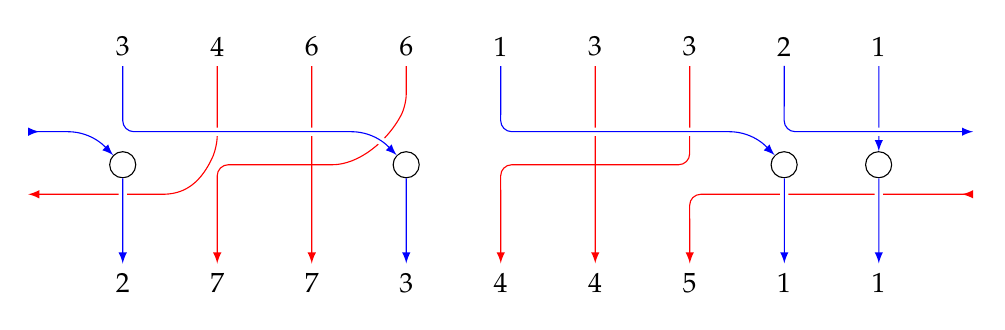
\begin{tikzpicture}[>=latex,rounded corners,yscale=1.5,xscale=1.2,baseline=0]
\def\passwidth{3pt};
\node (i1) at (1,1) {$3$};
\node (i2) at (2,1) {$4$};
\node (i3) at (3,1) {$6$};
\node (i4) at (4,1) {$6$};
\node (i5) at (5,1) {$1$};
\node (i6) at (6,1) {$3$};
\node (i7) at (7,1) {$3$};
\node (i8) at (8,1) {$2$};
\node (i9) at (9,1) {$1$};
\node (t1) at (1,-1) {$2$};
\node (t2) at (2,-1) {$7$};
\node (t3) at (3,-1) {$7$};
\node (t4) at (4,-1) {$3$};
\node (t5) at (5,-1) {$4$};
\node (t6) at (6,-1) {$4$};
\node (t7) at (7,-1) {$5$};
\node (t8) at (8,-1) {$1$};
\node (t9) at (9,-1) {$1$};
\node[circle,draw=black] (q1) at (1,0) {};
\node[circle,draw=black] (q2) at (4,0) {};
\node[circle,draw=black] (q3) at (8,0) {};
\node[circle,draw=black] (q4) at (9,0) {};
\draw[->,red] (i3) -- (t3);
\draw[->,red] (i4) -- (4,0.5) .. controls (3.8,0.2) and (3.5,0) .. (3.1,0) -- (2,0) -- (t2);
\draw[->,red] (i2) -- (2,0.15) .. controls (1.8,-0.2) and (1.6,-0.25) .. (1.3,-0.25) -- (0,-0.25);
\draw[>->,red] (10,-0.25) -- (8,-0.25) -- (7,-0.25) -- (t7);
\draw[->,red] (i6) -- (t6);
\draw[->,red] (i7) -- (7,0) -- (5,0) -- (t5);
\draw[white,line width=\passwidth] (5,0.28) -- (7.3,0.28) .. controls (7.7,0.28) and (7.85,0.12) .. (q3);  % To simulate underpass
\draw[->,blue] (i5) -- (5,0.28) -- (7.3,0.28) .. controls (7.7,0.28) and (7.85,0.12) .. (q3);
\draw[white,line width=\passwidth] (q3) -- (t8);  % To simulate underpass
\draw[->,blue] (q3) -- (t8);
\draw[->,blue] (i9) -- (q4);
\draw[white,line width=\passwidth] (q4) -- (t9);  % To simulate underpass
\draw[->,blue] (q4) -- (t9);
\draw[white,line width=\passwidth] (1,0.28) -- (3.3,0.28) .. controls (3.7,0.28) and (3.85,0.12) .. (q2);  % To simulate underpass
\draw[->,blue] (i1) -- (1,0.28) -- (3.3,0.28) .. controls (3.7,0.28) and (3.85,0.12) .. (q2);
\draw[->,blue] (q2) -- (t4);
\draw[white,line width=\passwidth] (i8) -- (8,0.28) -- (10,0.28);  % To simulate underpass
\draw[->,blue] (i8) -- (8,0.28) -- (10,0.28);
\draw[>->,blue] (0,0.28) -- (0.3,0.28) .. controls (0.7,0.28) and (0.85,0.12) .. (q1);
\draw[white,line width=\passwidth] (q1) -- (t1);  % To simulate underpass
\draw[->,blue] (q1) -- (t1);
\end{tikzpicture}
\]
where the paths in red correspond to Phase I and those in blue are from Phase
II (and where we have picked the permutation $\left(  i_{1}, i_{2}, \ldots,
i_{n} \right)  = \left(  5, 9, 8, 1, 7, 6, 2, 4, 3 \right)  $). Hence, we have
$q(346613321) = 277344511$, which has type $(2,1,1,2,1,0,2,\ldots)$.
\end{example}

We illustrate the situation $v = q(u)$ with a $2 \times n$ array, where the
first row is the word $u$ and the second row has a circle labeled $v_{j}$ for
$j \in q$ or a square labeled $v_{j}$ for $j \notin q$ in position $j$. Using
this convention, we can write Example~\ref{ex:first_queue} as
\[
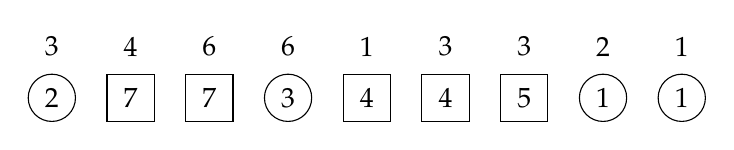
\begin{tikzpicture}[baseline=10]
\def\ll{0.65}   % level 2
\foreach \i in {5,9} { \node at (\i,\ll) {$1$}; }
\foreach \i in {8} { \node at (\i,\ll) {$2$}; }
\foreach \i in {1,6,7} { \node at (\i,\ll) {$3$}; }
\foreach \i in {2} { \node at (\i,\ll) {$4$}; }
\foreach \i in {3,4} { \node at (\i,\ll) {$6$}; }
\foreach \i in {1,4,8,9} { \draw (\i,0) circle (0.3); }
\foreach \i in {2,3,5,6,7} { \draw (\i-.3,0-.3) rectangle +(0.6,+0.6); }
\foreach \i in {8,9} { \node at (\i,0) {$1$}; }
\foreach \i in {1} { \node at (\i,0) {$2$}; }
\foreach \i in {4} { \node at (\i,0) {$3$}; }
\foreach \i in {5,6} { \node at (\i,0) {$4$}; }
\foreach \i in {7} { \node at (\i,0) {$5$}; }
\foreach \i in {2,3} { \node at (\i,0) {$7$}; }
\end{tikzpicture}
\]


\begin{comment}  % s-flow only seems to be used in this paragraph
Consider a pair $k, k+1 \pmod{n}$ of consecutive columns.
For $s > t$ the \defn{$s$-flow} from $k+1$ to $k$ is the number of $i$ such that $u_i=s$, and whose queueing interval $\inter[j,i]$ contains both $k$ and $k+1$.
Similarly, for $s < t$, the \defn{$s$-flow} from $k$ to $k+1$ is the number of $i$ such that $u_i = s$, and whose queueing interval $\inter[i,j]$ contains both $k$ and $k+1$.
\end{comment}


There is a natural duality in the algorithm above. For each queue $q$, let
$q^{*}$ be the {\color{darkred}\emph{contragredient dual queue}}, defined by
$\left(  i \in q^{*} \right)  \Longleftrightarrow\left(  n+1-i \notin q
\right)  $. Similarly, for each word $u$ with $\ell$ classes, let $u^{*}$ be
the {\color{darkred}\emph{contragredient dual word}} defined by $u^{*}_{i} =
\ell+ 1 - u_{n+1-i}$. For a fixed $k \in\left[  \ell\right]  $, we call $\ell+
1 - k$ the {\color{darkred}\emph{contragredient dual letter}} of $k$. Note
that if $q$ is an $r$-queue, then $q^{*}$ is the $(n-r)$-queue obtained by
reflecting $[n] \setminus q$ through the middle of $[n]$. Similarly, $u^{*}$
is obtained by reversing the word $u$ and taking the contragredient dual letters.

\begin{lemma}
[Contragredient duality]\label{le:dual} Let $q$ be a queue and $u$ be a word
with $\ell$ classes. Then we have $\bigl(q(u) \bigr)^{*} = q^{*}(u^{*})$,
\textit{i.e.}, we have $q(u)_{i} = \ell+ 2 - q^{*}(u^{*})_{n+1-i}$ for all $i$.
\end{lemma}

Here, we treat $q(u)$ as a word with $\ell+1$ classes, even if it may have
only $\ell$ classes (in the degenerate case when $q = \left[  n \right]  $).

\begin{proof}
Phase~I (resp.~II) in the construction of $q(u)$ corresponds to Phase~II
(resp.~I) in the construction of $q^{*}(u^{*})$ when the word is reversed and
the letters are replaced by their contragredient duals. Hence the claim follows.
\end{proof}

%\begin{remark} (Excision)
%Fix a queue $q$ and a word $u$, and let $i,j$ be columns. Suppose that the $s$-flow from $j+1$ to $j$ equals the $s$-flow from $i+1$ to $i$ for each $s > t$, and that the $s$-flow from $i$ to $i+1$ equals the $s$-flow from $j$ to $j+1$ for each $s < t$. Then we have $q_{|\inter[i,j]^c}(u_{|\inter[i,j]^c}) = \bigl( q(u) \bigr)_{|\inter[i,j]^c}$. Here, for a (cyclic) word $u$, we let $u_{|\inter[i,j]^c}$ denote the (cyclic) word gotten from simply removing the closed (cyclic) interval $\inter[i,j]$, and similarly for $q_{|\inter[i,j]^c}$.
%\end{remark}


%%%%%%%%%%


\subsection{Multiline queues}

We now give our main definition of a multiline queue and spectral weight.

\begin{dfn}
For $\sigma\in\mathfrak{S}_{\ell-1}$, a {\color{darkred}\emph{$\sigma$-twisted
multiline queue (MLQ) of type $\mathbf{m} = \left(  m_{1}, m_{2}, \ldots,
m_{\ell}, 0, 0, \ldots\right)  $}}, with $\ell$ classes, is a sequence of
queues $\mathbf{q} = (q_{1}, \dotsc, q_{\ell-1})$ such that $q_{i}$ is a
$p_{\sigma(i)}(\mathbf{m})$-queue and $m_{\ell} = n - p_{\ell-1}(\mathbf{m})$
(that is, $p_{\ell}(\mathbf{m}) = n$). When $\sigma$ is the identity
permutation, we simply call $\mathbf{q}$ an {\color{darkred}\emph{(ordinary)
MLQ of type $\mathbf{m}$}}. We also consider $\mathbf{q}$ as a function on
words by
\[
\mathbf{q}(u) := q_{\ell-1}\bigl( \cdots q_{2}\bigl( q_{1}(u) \bigr) \cdots
\bigr).
\]

\end{dfn}

\begin{remark}
Our notion of an (ordinary) MLQ is equivalent to what is called a ``discrete
MLQ'' in~\cite[\S 2.2]{AasLin17}, where we recover the labelling of level $k$
by $q_{k}( \cdots q_{1}(1 \dotsm1) \cdots)$. We omit the word ``discrete'' as
these are the only MLQs in this note.
\end{remark}

We shall now introduce generating functions for queues.

\begin{dfn}
Let $\mathbf{x} := \{x_{1}, x_{2}, x_{3}, \ldots\}$ be commuting indeterminates.

The {\color{darkred}\emph{weight}} of a queue $q$ is $\wt(q) := \prod_{i \in
q} x_{i}$.

The {\color{darkred}\emph{weight}} of a $\sigma$-twisted MLQ $\mathbf{q} =
(q_{1}, \dotsc, q_{\ell-1})$ is $\wt(\mathbf{q}) := \prod_{i=1}^{\ell-1}
\wt(q_{i})$.
\end{dfn}

\begin{dfn}
For $\sigma\in\mathfrak{S}_{\ell-1}$ and a packed word $u$ of type
$\mathbf{m}$ with $\ell$ classes, we define the {\color{darkred}\emph{$\sigma
$-spectral weight}} or {\color{darkred}\emph{$\sigma$-amplitude}} as
\begin{equation}
\label{eq:amplitude}\left\langle u \right\rangle _{\sigma} := \sum
_{\mathbf{q}} \wt(\mathbf{q}),
\end{equation}
where the sum is over all $\sigma$-twisted MLQs $\mathbf{q}$ of type
$\mathbf{m}$ satisfying $u = \mathbf{q}(1 \dotsm1)$. (Here, $1 \dotsm1$
denotes the word in $\mathcal{W}_{n}$ whose all letters are $1$.) When
$\sigma= \id$ is the identity permutation, we simply call this the
{\color{darkred}\emph{spectral weight}} or {\color{darkred}\emph{amplitude}}
and denote it by $\left\langle u \right\rangle := \left\langle u \right\rangle
_{\id}$.
\end{dfn}

\begin{remark}
\label{rmk:mlq-type} Let $\ell\geq1$ and $\sigma\in\mathfrak{S}_{\ell-1}$. Let
$\mathbf{q}$ be a $\sigma$-twisted MLQ. Then, the type of the word
$\mathbf{q}(1 \dotsm1)$ is the type of $\mathbf{q}$.
\end{remark}

\begin{proof}
Write the $\sigma$-twisted MLQ $\mathbf{q}$ as $\left(  q_{1}, \ldots,
q_{\ell-1} \right)  $. Let $\mathbf{m} = \left(  m_{1}, m_{2}, \ldots,
m_{\ell}, 0, 0, \ldots\right)  $ be the type of $\mathbf{q}$. Thus, $m_{1} +
m_{2} + \cdots+ m_{\ell}= p_{\ell}(\mathbf{m}) = n$. Now, the word $1 \dotsm1$
has type $\left(  n, 0, 0, \ldots\right)  = \left(  m_{1} + m_{2} + \cdots+
m_{\ell}, 0, 0, \ldots\right)  $ (since $n = m_{1} + m_{2} + \cdots+ m_{\ell}%
$). Every time we apply one of the queues $q_{i}$ to this word, the type
changes in a simple way: Namely, the plus sign between $m_{\sigma(i)}$ and
$m_{\sigma(i)+1}$ turns into a comma (so, for example, the application of
$q_{1}$ transforms it into $\left(  m_{1} + m_{2} + \cdots+ m_{\sigma(1)},
m_{\sigma(1)+1} + m_{\sigma(1)+2} + \cdots+ m_{\ell}, 0, 0, \ldots\right)  $).
Hence, the action of $\mathbf{q}$ transforms $1 \dotsm1$ into a word whose
type has all the plus signs replaced by commas -- \textit{i.e.}, whose type is
$\left(  m_{1}, m_{2}, \ldots, m_{\ell}, 0, 0, \ldots\right)  = \mathbf{m}$.
In other words, the type of the word $\mathbf{q}(1 \dotsm1)$ is $\mathbf{m}$.
\end{proof}

\todo[size=\tiny,inline,color=red!30]{The above proof -- which I don't find obvious -- is a bit informal. To make it more rigorous would take me another definition -- the ``p-sequence'' of a type $\mm$, which is defined to be $\tup{p_0(\mm), p_1(\mm), p_2(\mm), \ldots}$ (and which uniquely determines $\mm$). Using this p-sequence, we observe that the action of a queue on a word merely inserts the size of the queue into the p-sequence at the appropriate position (``insort''), so by applying $\qq$ to $11\cdots 1$ we will end up with a word that has the same p-sequence as $\mm$ and therefore the type $\mm$.
\\ \hfill --- Darij}
\todo[size=\tiny,inline,color=blue!30]{This is really just repeated applications of~\eqref{eq:queue_type_change} and induction on the number of queues.
\\ \hfill --- Travis}

\begin{remark}
Let $\ell\geq1$ and $\sigma\in\mathfrak{S}_{\ell-1}$. Let $u$ be a packed word
with $\ell$ classes and type $\mathbf{m}$. Then, there exists at least once
MLQ $\mathbf{q}$ of type $\mathbf{m}$ satisfying $\mathbf{q}(1 \dotsm1) = u$.
In other words, $\left\langle u \right\rangle \neq0$ (as a polynomial over
$\mathbb{Z}$).
\end{remark}

\begin{proof}
For each $k \in\left[  \ell-1 \right]  $, let $q_{k}$ be the set of all sites
$i$ such that $u_{i} \leq k$. It is then easy to check that $\mathbf{q} :=
\left(  q_{1}, q_{2}, \ldots, q_{\ell-1} \right)  $ is an MLQ of type
$\mathbf{m}$ satisfying $\mathbf{q}(1 \dotsm1) = u$.
\end{proof}

%%%%%%%%%%


\subsection{Symmetric polynomials}

We also need the {\color{darkred}\emph{elementary symmetric polynomials}} and
{\color{darkred}\emph{complete homogeneous symmetric polynomials}}. Recall
that they are defined for each $N \in\left\{  0,1,\ldots,n\right\}  $ and $k
\geq0$ by
\begin{align*}
e_{k}(x_{1}, x_{2}, \dotsc, x_{N})  &  = \sum_{1 \leq i_{1} < \cdots< i_{k}
\leq N} x_{i_{1}} \dotsm x_{i_{k}},\\
h_{k}(x_{1}, x_{2}, \dotsc, x_{N})  &  = \sum_{1 \leq i_{1} \leq\cdots\leq
i_{k} \leq N} x_{i_{1}} \dotsm x_{i_{k}},
\end{align*}
respectively. We define $e_{k}(x_{1}, \dotsc, x_{N}) = 0$ and $h_{k}(x_{1},
\dotsc, x_{N}) = 0$ for $k < 0$. For more details on symmetric polynomials, we
refer the reader to~\cite[Ch.~7]{Stanley-EC2}.

%=====================================================================


\section{Main results}

\label{sec:result}

In this section, we state our main results and use them to prove the
commutativity conjecture of~\cite{AAMP} and~\cite[Conj.~3.10]{AasLin17}.

\begin{thm}
\label{thm:permutation} Let $u$ be a packed word of type $\mathbf{m}$ with
$\ell$ classes. For any $\sigma\in\mathfrak{S}_{\ell-1}$, we have
\[
\left\langle u \right\rangle = \left\langle u \right\rangle _{\sigma}.
\]

\end{thm}

We will give the proof of Theorem~\ref{thm:permutation} in
Section~\ref{sec:thm_proof}. In order to prove our next result, we need the following.

If $w$ is a word of type $\mathbf{m}$, and if $j \geq0$, then $p_{j}%
(\mathbf{m})$ is the number of letters $\leq j$ in $w$.

For a word $w$ and a nonnegative integer $k$, we let
{\color{darkred}\emph{$\vee^{(k)} w$}} be the word obtained from $w$ by
decrementing (by $1$) all but the $k$ smallest letters of $w$. This is only
well-defined if these $k$ smallest letters are determined uniquely and the
remaining $n-k$ letters are $> 1$. In other words, this is only well-defined
if $k \in\left\{  p_{j}(\mathbf{m}) \mid j \geq1 \right\}  $, where
$\mathbf{m}$ is the type of $w$. Note that $\vee^{(k)} w = \vee_{j} w$, where
$j$ is such that $k = p_{j}(\mathbf{m})$.
%Note that $j$ is not necessarily unique, in which case $w$ is not a packed word, but the result is independent of the choice of $j$.


%\Travis{I am becoming less convinced of this notation as it makes things less explicit.
%Well-definedness is equivalent to the existence of a $j$ such that $p_j(\mm) = k$, and we really want to do the $j$-merge.
%It might be a little extra verbage, but I feel like it means more details and concepts are on the surface.}


\begin{lemma}
\label{lemma:queue_merge_commute} Let $u \in\mathcal{W}_{n}$ be a word of type
$\mathbf{m}$. Let $k \in\left\{  p_{j}(\mathbf{m}) \mid j \geq1 \right\}  $.
If $q$ is a queue, then
\[
\vee^{(k)} q(u) = q(\vee^{(k)} u).
\]
In particular, both $\vee^{(k)} q(u)$ and $\vee^{(k)} u$ are well-defined.
\end{lemma}

\begin{proof}
The word $\vee^{(k)} u$ is well-defined since $k = p_{j}(\mathbf{m})$ for some
$j \geq1$; furthermore, $\vee^{(k)} q(u)$ is well-defined since the type
$\mathbf{n}$ of $q(u)$ satisfies
\[
k \in\left\{  p_{j}(\mathbf{m}) \mid j \geq1 \right\}  \subseteq\left\{
p_{j}(\mathbf{m}) \mid j \geq1 \right\}  \cup\left\{  \left|  q \right|
\right\}  = \left\{  p_{j}(\mathbf{n}) \mid j \geq1 \right\}  .
\]
Thus, it remains to prove $\vee^{(k)} q(u) = q(\vee^{(k)} u)$. The permutation
$\left(  i_{1}, i_{2}, \dotsc, i_{n} \right)  $ in the construction of $q(u)$
also works for the construction of $q(\vee^{(k)} u)$, since $(\vee^{(k)}
u)_{a} \leq(\vee^{(k)} u)_{b}$ whenever $u_{a} \leq u_{b}$. Consequently, the
construction of $q(\vee^{(k)} u)$ proceeds exactly like the construction of
$q(u)$ (with the same entries being set in the same order), except that all
but the $k$ smallest letters are now smaller by $1$. Hence, $q(\vee^{(k)} u)$
is obtained from $q(u)$ by decrementing (by $1$) all but the $k$ smallest
letters of $q(u)$.
%(since $\vee^{(k)} u$ is obtained in this way from $u$).
However, the word $\vee^{(k)} q(u)$ is obtained from $q(u)$ in exactly the
same way. Therefore, we have $\vee^{(k)} q(u) = q(\vee^{(k)} u)$ as claimed.
\end{proof}

\begin{example}
Consider $q = \left\{  1,4,5,9,10 \right\}  $ and $v = 3455313321$:
\[
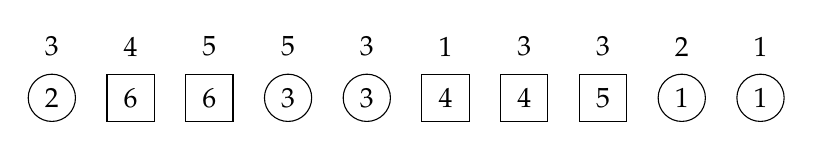
\begin{tikzpicture}[baseline=-7]
\def\ll{0.65}   % level 2
\foreach \i in {6,10} { \node at (\i,\ll) {$1$}; }
\foreach \i in {9} { \node at (\i,\ll) {$2$}; }
\foreach \i in {1,5,7,8} { \node at (\i,\ll) {$3$}; }
\foreach \i in {2} { \node at (\i,\ll) {$4$}; }
\foreach \i in {3,4} { \node at (\i,\ll) {$5$}; }
\foreach \i in {1,4,5,9,10} { \draw (\i,0) circle (0.3); }
\foreach \i in {2,3,6,7,8} { \draw (\i-.3,0-.3) rectangle +(0.6,+0.6); }
\foreach \i in {9,10} { \node at (\i,0) {$1$}; }
\foreach \i in {1} { \node at (\i,0) {$2$}; }
\foreach \i in {4,5} { \node at (\i,0) {$3$}; }
\foreach \i in {6,7} { \node at (\i,0) {$4$}; }
\foreach \i in {8} { \node at (\i,0) {$5$}; }
\foreach \i in {2,3} { \node at (\i,0) {$6$}; }
\end{tikzpicture}\ .
\]
Let $u = 3566413321$, and note that $v = \vee_{3} u = \vee^{(6)} u$ and
\[
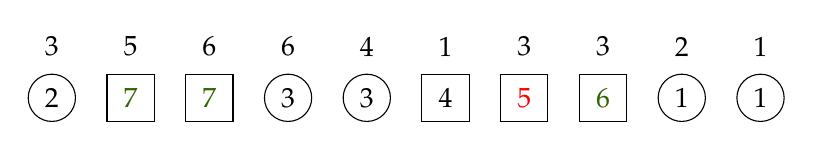
\begin{tikzpicture}[baseline=-7]
\def\ll{0.65}   % level 2
\foreach \i in {6,10} { \node at (\i,\ll) {$1$}; }
\foreach \i in {9} { \node at (\i,\ll) {$2$}; }
\foreach \i in {1,7,8} { \node at (\i,\ll) {$3$}; }
\foreach \i in {5} { \node at (\i,\ll) {$4$}; }
\foreach \i in {2} { \node at (\i,\ll) {$5$}; }
\foreach \i in {3,4} { \node at (\i,\ll) {$6$}; }
\foreach \i in {1,4,5,9,10} { \draw (\i,0) circle (0.3); }
\foreach \i in {2,3,6,7,8} { \draw (\i-.3,0-.3) rectangle +(0.6,+0.6); }
\foreach \i in {9,10} { \node at (\i,0) {$1$}; }
\foreach \i in {1} { \node at (\i,0) {$2$}; }
\foreach \i in {4,5} { \node at (\i,0) {$3$}; }
\foreach \i in {6} { \node at (\i,0) {$4$}; }
\foreach \i in {7} { \node[red] at (\i,0) {$5$}; }
\foreach \i in {8} { \node[dgreencolor] at (\i,0) {$6$}; }
\foreach \i in {2,3} { \node[dgreencolor] at (\i,0) {$7$}; }
\end{tikzpicture}\ ,
\]
where we have $2663344511 = \vee_{4} 2773345611 = \vee^{(6)} 2773345611$.
Similarly, let $u^{\prime}= 4566413421$, and note that $v = \vee_{3}
u^{\prime}$ and
\[
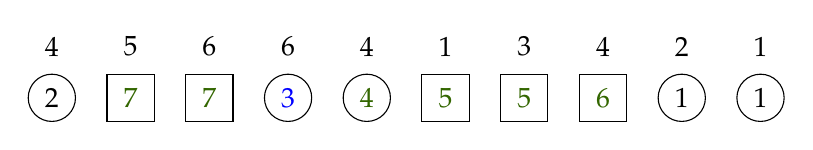
\begin{tikzpicture}[baseline=-7]
\def\ll{0.65}   % level 2
\foreach \i in {6,10} { \node at (\i,\ll) {$1$}; }
\foreach \i in {9} { \node at (\i,\ll) {$2$}; }
\foreach \i in {7} { \node at (\i,\ll) {$3$}; }
\foreach \i in {1,5,8} { \node at (\i,\ll) {$4$}; }
\foreach \i in {2} { \node at (\i,\ll) {$5$}; }
\foreach \i in {3,4} { \node at (\i,\ll) {$6$}; }
\foreach \i in {1,4,5,9,10} { \draw (\i,0) circle (0.3); }
\foreach \i in {2,3,6,7,8} { \draw (\i-.3,0-.3) rectangle +(0.6,+0.6); }
\foreach \i in {9,10} { \node at (\i,0) {$1$}; }
\foreach \i in {1} { \node at (\i,0) {$2$}; }
\foreach \i in {4} { \node[blue] at (\i,0) {$3$}; }
\foreach \i in {5} { \node[dgreencolor] at (\i,0) {$4$}; }
\foreach \i in {6,7} { \node[dgreencolor] at (\i,0) {$5$}; }
\foreach \i in {8} { \node[dgreencolor] at (\i,0) {$6$}; }
\foreach \i in {2,3} { \node[dgreencolor] at (\i,0) {$7$}; }
\end{tikzpicture}\ ,
\]
where we have $2663344511 = \vee_{4} 2773455611$.
\end{example}

\begin{lemma}
\label{lemma:queue_merge} Let $q^{\prime}$ be a $p_{i}(\mathbf{m})$-queue for
some type $\mathbf{m}$ and some $i \geq1$. Let the type $\mathbf{m}$ have
$\ell$ classes, and let $\sigma\in\mathfrak{S}_{\ell-1}$.
%be such that $\sigma(j) = j$ for all $j \geq i$.
Let $\mathbf{q}$ be a $\sigma$-twisted MLQ of type $\vee_{i}\mathbf{m}$.
%Darij: Yes, we need $\sigma$-twisted here, due to how we apply this
%lemma repeatedly in the proof of Theorem \ref{thm:determinant_form}.
%(To apply it repeatedly, we need $\sigma$-twisted MLQs, since an
%MLQ might become $\sigma$-twisted after the first application.)
For the word $u = \mathbf{q}\bigl( q^{\prime}(1 \dotsm1) \bigr), $ we have
\[
\mathbf{q}(1 \dotsm1) = \vee_{i} u.
\]

\end{lemma}

\begin{proof}
\begin{comment}
Let us first show an auxiliary observation.
Let $q$, $u$ and $t$ be as in Remark~\ref{rmk:t-splitting},
and let $h \in \set{1, 2, \ldots}$.
The permutation $\tup{i_1, i_2, \ldots, i_n}$ in the construction of $q(u)$
also works for the construction of $q(\merge{h} u)$,
since $(\merge{h} u)_a \leq (\merge{h} u)_b$ whenever $u_a \leq u_b$.
Thus, the construction of $q(\merge{h} u)$ proceeds exactly as the
construction of $q(u)$, except that the letters used to build
the former word are those of $\merge{h} u$ instead of those of $u$.
This yields an expression for each letter $(q(\merge{h} u))_i$ of
$q(\merge{h} u)$ depending on whether ...
\begin{equation}
q(\merge{h} u) = \begin{cases}
\merge{h} q(u) , & \text{ if } h < t ; \\
\merge{h+1} q(u) , & \text{ if } h \geq t
\end{cases} .
\label{pf.lemma:queue_merge.1}
\end{equation}
\end{comment}
Write the $\sigma$-twisted MLQ $\mathbf{q}$ as $\left(  q_{1}, \ldots,
q_{\ell-1} \right)  $. It has type $\vee_{i} \mathbf{m}$.

%Thus, the queue $q_j$ has size
%$p_{\sigma(j)}(\merge{i} \mm) = p_{\sigma(j)}(\mm)$
%for each $j < i$
%(here, we have used the fact that $j < i$ entails
%$\sigma(j) < i$;
%this is a consequence of our assumption on $\sigma$),
%and size
%$p_{\sigma(j)}(\merge{i} \mm) = p_j(\merge{i} \mm) = p_{j+1}(\mm)$
%for each $j \geq i$.


%The permutation
%$\zeta := s_{i-1} \cdots s_2 s_1 \in \SymGp{\ell-1}$ is the
%$i$-cycle sending $1, 2, \ldots, i$ to $i, 1, 2, \ldots, i-1$.
Set $\mathbf{q}^{\prime}:= \left(  q^{\prime}, q_{1}, \ldots, q_{\ell-1}
\right)  $; this is easily seen to be a $\zeta$-twisted MLQ of type
$\mathbf{m}$, for some $\zeta\in\mathfrak{S}_{\ell}$ (since the multiset of
the $p_{k}(\vee_{i}\mathbf{m})$ for $k \geq1$ is precisely the multiset of the
$p_{k}(\mathbf{m})$ for $k \geq1$ with one copy of $p_{i}(\mathbf{m}) =
\left|  q^{\prime}\right|  $ removed). Furthermore, the definition of $u$
becomes $u = \mathbf{q}^{\prime}(1 \dotsm1)$. Hence, the type of $u$ is
$\mathbf{m}$ (by Remark~\ref{rmk:mlq-type}).

Set $k = p_{i}(\mathbf{m})$. Then, $q^{\prime}$ is a $k$-queue, so that the
type $\mathbf{n}$ of the word $q(1 \dots1)$ satisfies $p_{1}(\mathbf{n}) = k$.
Hence, any word obtained by actions of queues on $q^{\prime}(1 \dots1)$ will
have its type $\mathbf{n}$ satisfy $k \in\left\{  p_{j}(\mathbf{n}) \mid j
\geq0 \right\}  $.

Since the type of $u$ is $\mathbf{m}$, and since $k = p_{i}(\mathbf{m})$, we
have
\begin{equation}
\label{pf.lemma:queue_merge.4}\vee_{i} u = \vee^{(k)} (u) = \vee^{(k)}
\mathbf{q}\bigl( q^{\prime}(1 \dotsm1) \bigr) = \mathbf{q}\bigl( \vee^{(k)}
q^{\prime}(1 \dotsm1) \bigr)
\end{equation}
by repeated use of Lemma~\ref{lemma:queue_merge_commute} (since any word
obtained by actions of queues on $q^{\prime}(1 \dotsm1)$ will have its type
$\mathbf{n}$ satisfy $k \in\left\{  p_{j}(\mathbf{n}) \mid j \geq1 \right\}
$). It is clear that $\vee^{(k)} q^{\prime}(1 \dotsm1) = 1 \dotsm1$, and
so~\eqref{pf.lemma:queue_merge.4} becomes $\mathbf{q}(1 \dotsm1) = \vee_{i} u$.
\end{proof}

\begin{thm}
\label{thm:merge} Let $\mathbf{m}$ be a type with $m_{i} \neq0$ and $m_{i+1}
\neq0$. Let $v$ be a packed word of type $\vee_{i}\mathbf{m}$. Then,
\[
\left\langle v \right\rangle e_{p_{i}(\mathbf{m})}(x_{1}, \dotsc, x_{n}) =
\sum_{u} \left\langle u \right\rangle ,
\]
where we sum over all $u$ of type $\mathbf{m}$ such that $v = \vee_{i} u$.
\end{thm}

\begin{proof}
The type $\mathbf{m}$ is packed (since $m_{i} \neq0$ and $m_{i+1} \neq0$, and
since $\vee_{i}\mathbf{m}$ is packed). Let $\vee_{i}\mathbf{m}$ have $\ell$
classes; then, $\mathbf{m}$ has $\ell+1$ classes. First note that
\[
\left\langle v \right\rangle e_{p_{i}(\mathbf{m})}(x_{1}, \dotsc, x_{n}) =
\sum_{(\mathbf{q},q^{\prime})} \wt(\mathbf{q}) \wt(q^{\prime}),
\]
where we sum over all pairs $(\mathbf{q}, q^{\prime})$ such that

\begin{itemize}
\item $\mathbf{q} = (q_{1}, \dotsc, q_{\ell-1})$ is an MLQ of type $\vee
_{i}\mathbf{m}$ such that $v = \mathbf{q}(1\cdots1)$ and

\item $q^{\prime}$ is a $p_{i}(\mathbf{m})$-queue.
\end{itemize}

Given any such pair $\left(  \mathbf{q}, q^{\prime}\right)  $, we set
\[
\theta(\mathbf{q}, q^{\prime}) := (q^{\prime}, q_{1}, \dotsc, q_{\ell-1});
\]
the result is a $(s_{i-1} \dotsm s_{2} s_{1})$-twisted MLQ of type
$\mathbf{m}$ with weight $\wt\bigl( \theta(\mathbf{q}, q^{\prime}) \bigr) =
\wt(\mathbf{q}) \wt(q^{\prime})$. But recall that $v = \mathbf{q}(1 \dotsm1$);
thus, by Lemma~\ref{lemma:queue_merge}, we have
\[
v = \mathbf{q}(1 \dotsm1) = \vee_{i} \mathbf{q}\bigl( q^{\prime}(1 \dotsm1)
\bigr) = \vee_{i} \bigl( \theta(\mathbf{q}, q^{\prime})(1 \dotsm1) \bigr).
\]
Thus, we have defined a weight preserving bijection $\theta$ from the set of
all pairs $(\mathbf{q}, q^{\prime})$ as above to the set of all $(s_{i-1}
\dotsm s_{1})$-twisted MLQs $\widetilde{\mathbf{q}}$ of type $\mathbf{m}$
satisfying $v = \vee_{i} \widetilde{\mathbf{q}} \left(  1 \dotsm1 \right)  $.
Hence, we have
\[
\sum_{(\mathbf{q},q^{\prime})} \wt(\mathbf{q}) \wt(q^{\prime}) =
\sum_{\widetilde{\mathbf{q}}} \wt(\widetilde{\mathbf{q}}) = \sum_{u}
\left\langle u \right\rangle _{s_{i-1} \dotsm s_{1}} ,
\]
where the last sum is over all words $u$ of type $\mathbf{m}$ satisfying $v =
\vee_{i} u$. Finally, we have $\left\langle u \right\rangle _{s_{i-1} \dotsm
s_{1}} = \left\langle u \right\rangle $ for all such $u$ by
Theorem~\ref{thm:permutation}. Combining all the above equalities, we find
$\left\langle v \right\rangle e_{p_{i}(\mathbf{m})}(x_{1}, \dotsc, x_{n}) =
\sum_{u} \left\langle u \right\rangle $.
\end{proof}

\begin{remark}
\label{rmk:bijective_proof} Our proof of Theorem~\ref{thm:permutation} is by
constructing a bijection $\omega$, and hence, we can give a bijective proof of
Theorem~\ref{thm:merge} by the composition $\omega\circ\theta$.
\end{remark}

\begin{example}
Suppose $n = 5$. Let $v = 13234$, and we have that $v = \vee_{3} u$ if and
only if $u \in\left\{  13245, 14235 \right\}  $. By examining all possible
MLQs for these words, we obtain
\begin{align*}
\left\langle 13234 \right\rangle  &  = x_{1} x_{2} x_{3}^{2} x_{4} (x_{1}^{2}
+ x_{1} x_{4} + x_{1} x_{5} + x_{4} x_{5} + x_{5}^{2}),\\
\left\langle 13245 \right\rangle  &  = x_{1} x_{2} x_{3}^{2} x_{4} (x_{1}^{2}
+ x_{1}x_{4} + x_{1}x_{5} + x_{4}^{2} + x_{4}x_{5} + x_{5}^{2})\\
&  \hspace{20pt} \times(x_{1}x_{2}x_{3} + x_{1}x_{2}x_{5}+x_{1}x_{3}%
x_{5}+x_{2}x_{3}x_{5}),\\
\left\langle 14235 \right\rangle  &  = x_{1}x_{2}x_{3}^{2}x_{4}^{2} (x_{1}%
^{3}x_{2} + x_{1}^{3}x_{3} + x_{1}^{3}x_{5} + x_{1}^{2}x_{2}x_{3} + x_{1}%
^{2}x_{2}x_{4} + 2x_{1}^{2}x_{2}x_{5}\\
&  \hspace{60pt} + x_{1}^{2}x_{3}x_{4} + 2x_{1}^{2}x_{3}x_{5} + x_{1}^{2}%
x_{4}x_{5} + x_{1}^{2}x_{5}^{2} + x_{1}x_{2}x_{3}x_{5}\\
&  \hspace{60pt} + x_{1}x_{2}x_{4}x_{5} + 2x_{1}x_{2}x_{5}^{2} + x_{1}%
x_{3}x_{4}x_{5} + 2x_{1}x_{3}x_{5}^{2} + x_{1}x_{4}x_{5}^{2}\\
&  \hspace{60pt} + x_{1}x_{5}^{3} + x_{2}x_{3}x_{5}^{2} + x_{2}x_{4}x_{5}^{2}
+ x_{2}x_{5}^{3} + x_{3}x_{4}x_{5}^{2} + x_{3}x_{5}^{3}).
\end{align*}
(We have factored the expressions for readability only.) We verify
Theorem~\ref{thm:merge} in this case by computing $\left\langle 13234
\right\rangle e_{3}(x_{1}, x_{2}, x_{3}, x_{4}, x_{5}) = \left\langle 13245
\right\rangle + \left\langle 14235 \right\rangle $.
\end{example}

%=====================================================================


\section{A Jacobi-Trudi-like formula for special $u$}

\label{sec:JT_formula}

XBEGIN

The goal of this section is to prove a determinantal formula (Theorem
\ref{thm:determinant_form}) for $\left\langle u\right\rangle $ in the special
case when $u$ is a packed word with either $\ell-1$ or $\ell$ classes and
becomes weakly decreasing if we disregard all letters $\ell$. (For example,
$u={\color{gray}4}3{\color{gray}44}33{\color{gray}4}22{\color{gray}4}%
211{\color{gray}4}$ is such a word, with $\ell=4$.) This will then help us
settle two conjectures from \cite{AasLin17}.

Throughout this section, we shall regard the sites $1,2,\ldots,n$ as positive
integers rather than elements of $\mathbb{Z}/n\mathbb{Z}$. In particular, they
are totally ordered by $1<2<\cdots<n$. Moreover, we shall use infinitely many
distinct commuting indeterminates $\ldots,x_{-2},x_{-1},x_{0},x_{1}%
,x_{2},\ldots$ instead of the $n$ indeterminates $x_{1},x_{2},\ldots,x_{n}$;
thus, we don't have $x_{n+k}=x_{k}$ for $k\in\mathbb{Z}$ in this section.

\subsection{Lattice paths and the Lindstr\"{o}m--Gessel--Viennot theorem}

Our arguments will rely on the Lindstr\"om--Gessel--Viennot
Lemma~\cite{GV85,Lindstrom73} and on a re-interpretation of MLQs as a certain
kind of semistandard tableaux (of non-partition shape). This takes inspiration
from the \textquotedblleft bully paths\textquotedblright\ of~\cite{AasLin17}
as well as from the standard proof of the Jacobi--Trudi identities for Schur
functions~\cite[First proof of Theorem 7.16.1]{Stanley-EC2}. We begin with
basic definitions.

The \defn{lattice} shall mean the (infinite) directed graph whose vertices are
all pairs of integers (that is, its vertex set is $\mathbb{Z}^{2}$), and whose
arcs are
\begin{align*}
\left(  i,j\right)   &  \rightarrow\left(  i,j+1\right)  \qquad\text{for all
}\left(  i,j\right)  \in\mathbb{Z}\text{,}\qquad\text{and}\\
\left(  i,j\right)   &  \rightarrow\left(  i+1,j\right)  \qquad\text{for all
}\left(  i,j\right)  \in\mathbb{Z}\text{.}%
\end{align*}
The arcs of the first kind are called \defn{north-steps}, whereas the arcs of
the second kind are called \defn{east-steps}. The vertices of the lattice will
just be called \defn{vertices}. We draw the lattice as the usual integer
lattice in the Cartesian plane.

For each vertex $v=\left(  i,j\right)  $, we set $\operatorname*{x}\left(
v\right)  =i$ and $\operatorname*{y}\left(  v\right)  =j$. We refer to
$\operatorname*{x}\left(  v\right)  $ as the \defn{x-coordinate} of $v$, and
to $\operatorname*{y}\left(  v\right)  $ as the \defn{y-coordinate} of $v$.
The \defn{y-coordinate} of an east-step $\left(  i,j\right)  \rightarrow
\left(  i+1,j\right)  $ is defined to be $j$.

For each arc $a$ of the lattice, we define the
\defn{weight $\operatorname{wt}a$} of $a$ as the following monomial:%
\[
\operatorname*{wt}a=%
\begin{cases}
x_{j}, & \text{if }a\text{ is of the form }\left(  i,j\right)  \rightarrow
\left(  i+1,j\right)  ;\\
1, & \text{if }a\text{ is of the form }\left(  i,j\right)  \rightarrow\left(
i,j+1\right)  .
\end{cases}
\]
Thus, north-steps have weight $1$, while east-steps at y-coordinate $j$ have
weight $x_{j}$.

Fix $k\in\mathbb{N}$. A \defn{$k$-vertex} shall mean a $k$-tuple of vertices
of the lattice. If $\mathbf{v}=\left(  A_{1},A_{2},\ldots,A_{k}\right)  $ is a
$k$-vertex, and if $\sigma\in\mathfrak{S}_{k}$ is a permutation, then
$\sigma\left(  \mathbf{v}\right)  $ denotes the $k$-vertex $\left(
A_{\sigma\left(  1\right)  },A_{\sigma\left(  2\right)  },\ldots
,A_{\sigma\left(  k\right)  }\right)  $.

A \defn{path} will simply mean a (directed) path in the lattice. The
\defn{weight $\operatorname{wt}p$} of a path $p$ is defined as the product of
the weights of all arcs of this path; this weight is a monomial. If $A$ and
$B$ are two vertices, then \defn{$N\left(  A,B\right)$} shall denote the set
of all paths from $A$ to $B$.

If $\left(  A_{1},A_{2},\ldots,A_{k}\right)  $ and $\left(  B_{1},B_{2}%
,\ldots,B_{k}\right)  $ are two $k$-vertices, then a \defn{NILP} from $\left(
A_{1},A_{2},\ldots,A_{k}\right)  $ to $\left(  B_{1},B_{2},\ldots
,B_{k}\right)  $ shall mean a $k$-tuple $\left(  p_{1},p_{2},\ldots
,p_{k}\right)  $ of paths such that

\begin{itemize}
\item each $p_{i}$ is a path from $A_{i}$ to $B_{i}$;

\item no two of the paths $p_{1},p_{2},\ldots,p_{k}$ have a vertex in common.
\end{itemize}

(\textquotedblleft NILP\textquotedblright\ stands for \textquotedblleft
non-intersecting lattice paths\textquotedblright, but note that the paths must
neither cross nor touch.)

The \defn{weight $\operatorname{wt}\mathbf{p}$} of a NILP $\mathbf{p}=\left(
p_{1},p_{2},\ldots,p_{k}\right)  $ is defined as $\prod_{i=1}^{k}%
\operatorname*{wt}\left(  p_{i}\right)  $; this weight is a monomial.

TODO: Picture of a NILP with weight. Don't align the sources or targets on a line.

If $\mathbf{u}$ and $\mathbf{v}$ are two $k$-vertices, then
\defn{$N\left( \mathbf{u},\mathbf{v}\right)  $} denotes the set of all NILPs
from $\mathbf{u}$ to $\mathbf{v}$.

A pair $\left(  \mathbf{u},\mathbf{v}\right)  $ of two $k$-vertices
$\mathbf{u}$ and $\mathbf{v}$ is said to be \defn{nonpermutable} if and only
if every permutation $\sigma\neq\operatorname*{id}$ in $\mathfrak{S}_{k}$
satisfies $N\left(  \mathbf{u},\sigma\left(  \mathbf{v}\right)  \right)
=\varnothing$. Note that we are not requiring that $N\left(  \mathbf{u}%
,\mathbf{v}\right)  \neq\varnothing$ here.

The following fact (a particular case of \cite[Corollary 2]{GesVie89}) is crucial:

\begin{prop}
\label{prop.LGV.nonper}Let $k\in\mathbb{N}$. Let $\left(  \mathbf{u}%
,\mathbf{v}\right)  $ be a nonpermutable pair of two $k$-vertices
$\mathbf{u}=\left(  A_{1},A_{2},\ldots,A_{k}\right)  $ and $\mathbf{v}=\left(
B_{1},B_{2},\ldots,B_{k}\right)  $. Then,%
\[
\sum_{\mathbf{p}\in N\left(  \mathbf{u},\mathbf{v}\right)  }\operatorname*{wt}%
\mathbf{p}=\det\left(  \left(  \sum_{p\in N\left(  A_{i},B_{j}\right)
}\operatorname*{wt}p\right)  _{1\leq i\leq k,\ 1\leq j\leq k}\right)  .
\]

\end{prop}

It is also easy to see that any two vertices $A=\left(  a,b\right)  $ and
$B=\left(  c,d\right)  $ satisfy%
\begin{equation}
\sum_{p\in N\left(  A,B\right)  }\operatorname*{wt}p=h_{c-a}\left(
x_{b},x_{b+1},\ldots,x_{d}\right)  . \label{eq.LGV.single-paths}%
\end{equation}
(Here, $h_{\ell}\left(  x_{b},x_{b+1},\ldots,x_{d}\right)  $ is defined as
$\sum_{\substack{\left(  k_{1},k_{2},\ldots,k_{\ell}\right)  \in\left\{
b,b+1,\ldots,d\right\}  ^{\ell};\\k_{1}\leq k_{2}\leq\cdots\leq k_{\ell}%
}}x_{k_{1}}x_{k_{2}}\cdots x_{k_{\ell}}$ for all $\ell\in\mathbb{N}$, and is
$0$ otherwise.)

\begin{proof}
[Proof of \eqref{eq.LGV.single-paths}.]Let $A=\left(  a,b\right)  $ and
$B=\left(  c,d\right)  $ be two vertices. If $p$ is a path from $A$ to $B$,
then $p$ must have exactly $c-a$ east-steps, and the y-coordinates of these
east-steps must belong to the interval $\left\{  b,b+1,\ldots,d\right\}  $.
For any such path $p$, let $y_{1}\left(  p\right)  ,y_{2}\left(  p\right)
,\ldots,y_{c-a}\left(  p\right)  $ be the y-coordinates of the $c-a$
east-steps of $p$ (from left to right). Thus, $\left(  y_{1}\left(  p\right)
,y_{2}\left(  p\right)  ,\ldots,y_{c-a}\left(  p\right)  \right)  $ is a
weakly increasing $\left(  c-a\right)  $-tuple of elements of $\left\{
b,b+1,\ldots,d\right\}  $. Moreover, $p$ can be uniquely reconstructed from
this $\left(  c-a\right)  $-tuple (since these $\left(  c-a\right)  $-tuple
determines the east-steps of $p$). Conversely, any weakly increasing $\left(
c-a\right)  $-tuple of elements of $\left\{  b,b+1,\ldots,d\right\}  $ has the
form $\left(  y_{1}\left(  p\right)  ,y_{2}\left(  p\right)  ,\ldots
,y_{c-a}\left(  p\right)  \right)  $ for a unique path $p$ from $A$ to $B$.
Thus, there is a bijection between the paths $p$ from $A$ to $B$ and the
weakly increasing $\left(  c-a\right)  $-tuples of elements of $\left\{
b,b+1,\ldots,d\right\}  $. This yields
\[
\sum_{p\in N\left(  A,B\right)  }\operatorname*{wt}p=\sum_{\substack{\left(
k_{1},k_{2},\ldots,k_{c-a}\right)  \text{ is a weakly increasing}\\\left(
c-a\right)  \text{-tuple of elements of }\left\{  b,b+1,\ldots,d\right\}
}}x_{k_{1}}x_{k_{2}}\cdots x_{k_{c-a}}=h_{c-a}\left(  x_{b},x_{b+1}%
,\ldots,x_{d}\right)  .
\]

\end{proof}

Next, we state a simple lemma that will help us show that certain pairs of
$k$-vertices are nonpermutable:

\begin{lemma}
\label{lem.LGV.hex}Let $A$, $B$, $A^{\prime}$ and $B^{\prime}$ be four
vertices such that%
\[
\operatorname*{x}\left(  A^{\prime}\right)  \leq\operatorname*{x}\left(
A\right)  ,\qquad\operatorname*{y}\left(  A^{\prime}\right)  \geq
\operatorname*{y}\left(  A\right)  ,\qquad\operatorname*{x}\left(  B^{\prime
}\right)  \leq\operatorname*{x}\left(  B\right)  ,\qquad\operatorname*{y}%
\left(  B^{\prime}\right)  \geq\operatorname*{y}\left(  B\right)  .
\]
Let $p$ be a path from $A$ to $B^{\prime}$. Let $p^{\prime}$ be a path from
$A^{\prime}$ to $B$. Then, $p$ and $p^{\prime}$ have a vertex in common.
\end{lemma}

TODO: Example picture.

\begin{proof}
[First proof of Lemma \ref{lem.LGV.hex}.]If $q$ is any path, then the
\defn{length $\ell\left(q\right)$} of $q$ is defined to be the number of arcs
of $q$.

We shall now prove Lemma \ref{lem.LGV.hex} by strong induction on $\ell\left(
p\right)  +\ell\left(  p^{\prime}\right)  $:

\textit{Induction step:} Fix $N\in\mathbb{N}$. Assume (as the induction
hypothesis) that Lemma \ref{lem.LGV.hex} holds whenever $\ell\left(  p\right)
+\ell\left(  p^{\prime}\right)  <N$. We must now prove that Lemma
\ref{lem.LGV.hex} holds when $\ell\left(  p\right)  +\ell\left(  p^{\prime
}\right)  =N$.

So let $A$, $B$, $A^{\prime}$, $B^{\prime}$, $p$ and $p^{\prime}$ be as in
Lemma \ref{lem.LGV.hex}, and let us assume that $\ell\left(  p\right)
+\ell\left(  p^{\prime}\right)  =N$. We must prove that $p$ and $p^{\prime}$
have a vertex in common.

Assume the contrary. Thus, $p$ and $p^{\prime}$ have no vertex in common.

The vertex $A$ belongs to the path $p$, and thus does not belong to the path
$p^{\prime}$ (since $p$ and $p^{\prime}$ have no vertex in common). Similarly,
the vertex $A^{\prime}$ does not belong to the path $p$.

Recall that each arc of the lattice is either an east-step or a north-step.
Thus, the x-coordinates of the vertices of a path are always weakly
increasing, and so are the y-coordinates. Hence, the existence of a path $p$
from $A$ to $B^{\prime}$ shows that $\operatorname*{x}\left(  A\right)
\leq\operatorname*{x}\left(  B^{\prime}\right)  $ and $\operatorname*{y}%
\left(  A\right)  \leq\operatorname*{y}\left(  B^{\prime}\right)  $.
Similarly, the existence of a path $p^{\prime}$ from $A^{\prime}$ to $B$
yields $\operatorname*{x}\left(  A^{\prime}\right)  \leq\operatorname*{x}%
\left(  B\right)  $ and $\operatorname*{y}\left(  A^{\prime}\right)
\leq\operatorname*{y}\left(  B\right)  $.

Next, we claim that $\ell\left(  p\right)  \neq0$.

[\textit{Proof:} Assume the contrary. Thus, $\ell\left(  p\right)  =0$. Hence,
the path $p$ has no steps. Therefore, $A=B^{\prime}$ (since $p$ is a path from
$A$ to $B^{\prime}$). Hence, $\operatorname*{y}\left(  A\right)
=\operatorname*{y}\left(  B^{\prime}\right)  \geq\operatorname*{y}\left(
B\right)  $, so that $\operatorname*{y}\left(  A^{\prime}\right)
\geq\operatorname*{y}\left(  A\right)  \geq\operatorname*{y}\left(  B\right)
$. Combining this with $\operatorname*{y}\left(  A^{\prime}\right)
\leq\operatorname*{y}\left(  B\right)  $, we obtain $\operatorname*{y}\left(
A^{\prime}\right)  =\operatorname*{y}\left(  B\right)  $. Combining
$\operatorname*{y}\left(  A^{\prime}\right)  \geq\operatorname*{y}\left(
A\right)  $ with $\operatorname*{y}\left(  A^{\prime}\right)
=\operatorname*{y}\left(  B\right)  \leq\operatorname*{y}\left(  A\right)  $,
we obtain $\operatorname*{y}\left(  A^{\prime}\right)  =\operatorname*{y}%
\left(  A\right)  $. Thus, $\operatorname*{y}\left(  A^{\prime}\right)
=\operatorname*{y}\left(  A\right)  =\operatorname*{y}\left(  B\right)  $.
Therefore, the vertex $A$ lies on the horizontal line that contains
$A^{\prime}$ and $B$. Furthermore, this vertex $A$ must lie on the line
segment between $A^{\prime}$ and $B$ (since $\operatorname*{x}\left(
A^{\prime}\right)  \leq\operatorname*{x}\left(  \underbrace{A}_{=B^{\prime}%
}\right)  =\operatorname*{x}\left(  B^{\prime}\right)  \leq\operatorname*{x}%
\left(  B\right)  $).

Recall again that the y-coordinates of the vertices a path are always weakly
increasing. Moreover, they increase strictly whenever the path makes a
north-step. Hence, if the path $p^{\prime}$ would have any north-step, then we
would have $\operatorname*{y}\left(  A^{\prime}\right)  <\operatorname*{y}%
\left(  B\right)  $ (since $p^{\prime}$ is a path from $A^{\prime}$ to $B$).
But this would contradict $\operatorname*{y}\left(  A^{\prime}\right)
\geq\operatorname*{y}\left(  B\right)  $. Hence, the path $p^{\prime}$ has no
north-step. Thus, $p^{\prime}$ consists entirely of east-steps. Hence,
$p^{\prime}$ contains every vertex on the line segment between $A^{\prime}$
and $B$. Therefore, $p^{\prime}$ contains the vertex $A$ (since the vertex $A$
lies on the line segment between $A^{\prime}$ and $B$). This contradicts the
fact that $A$ does not belong to the path $p^{\prime}$. This contradiction
shows that our assumption was false; hence, $\ell\left(  p\right)  \neq0$ is proven.]

Furthermore, we claim that $\ell\left(  p^{\prime}\right)  \neq0$.

[\textit{Proof:} Assume the contrary. Thus, $\ell\left(  p^{\prime}\right)
=0$. Hence, the path $p^{\prime}$ has no steps. Therefore, $A^{\prime}=B$
(since $p^{\prime}$ is a path from $A^{\prime}$ to $B$). Hence,
$\operatorname*{x}\left(  A^{\prime}\right)  =\operatorname*{x}\left(
B\right)  \geq\operatorname*{x}\left(  B^{\prime}\right)  $, so that
$\operatorname*{x}\left(  A\right)  \geq\operatorname*{x}\left(  A^{\prime
}\right)  \geq\operatorname*{x}\left(  B^{\prime}\right)  $. Combining this
with $\operatorname*{x}\left(  A\right)  \leq\operatorname*{x}\left(
B^{\prime}\right)  $, we obtain $\operatorname*{x}\left(  A\right)
=\operatorname*{x}\left(  B^{\prime}\right)  $. Combining $\operatorname*{x}%
\left(  A\right)  \geq\operatorname*{x}\left(  A^{\prime}\right)  $ with
$\operatorname*{x}\left(  A^{\prime}\right)  \geq\operatorname*{x}\left(
B^{\prime}\right)  =\operatorname*{x}\left(  A\right)  $, we obtain
$\operatorname*{x}\left(  A\right)  =\operatorname*{x}\left(  A^{\prime
}\right)  $. Thus, $\operatorname*{x}\left(  A^{\prime}\right)
=\operatorname*{x}\left(  A\right)  =\operatorname*{x}\left(  B^{\prime
}\right)  $. Therefore, the vertex $A^{\prime}$ lies on the vertical line that
contains $A$ and $B^{\prime}$. Furthermore, this vertex $A^{\prime}$ must lie
on the line segment between $A$ and $B^{\prime}$ (since $\operatorname*{y}%
\left(  A^{\prime}\right)  \geq\operatorname*{y}\left(  A\right)  $ and
$\operatorname*{y}\left(  \underbrace{A^{\prime}}_{=B}\right)
=\operatorname*{y}\left(  B\right)  \leq\operatorname*{y}\left(  B^{\prime
}\right)  $).

Recall again that the x-coordinates of the vertices a path are always weakly
increasing. Moreover, they increase strictly whenever the path makes an
east-step. Hence, if the path $p$ would have any east-step, then we would have
$\operatorname*{x}\left(  A\right)  <\operatorname*{x}\left(  B^{\prime
}\right)  $ (since $p$ is a path from $A$ to $B^{\prime}$). But this would
contradict $\operatorname*{x}\left(  A\right)  =\operatorname*{x}\left(
B^{\prime}\right)  $. Hence, the path $p$ has no east-step. Thus, $p$ consists
entirely of north-steps. Hence, $p$ contains every vertex on the line segment
between $A$ and $B^{\prime}$. Therefore, $p$ contains the vertex $A^{\prime}$
(since the vertex $A^{\prime}$ lies on the line segment between $A$ and
$B^{\prime}$). This contradicts the fact that $A^{\prime}$ does not belong to
the path $p$. This contradiction shows that our assumption was false; hence,
$\ell\left(  p^{\prime}\right)  \neq0$ is proven.]

Let $P$ be the second vertex of the path $p$. (This is well-defined, since
$\ell\left(  p\right)  \neq0$.) Hence, $P$ lies on a path from $A$ to
$B^{\prime}$ (namely, on the path $p$). Therefore, $\operatorname*{x}\left(
A\right)  \leq\operatorname*{x}\left(  P\right)  \leq\operatorname*{x}\left(
B^{\prime}\right)  $ (since the x-coordinates of the vertices a path are
always weakly increasing) and $\operatorname*{y}\left(  A\right)
\leq\operatorname*{y}\left(  P\right)  \leq\operatorname*{y}\left(  B^{\prime
}\right)  $ (since the y-coordinates of the vertices a path are always weakly
increasing). Let $r$ be the path from $P$ to $B^{\prime}$ obtained by removing
the first arc from $p$. Thus, $r$ is a subpath of $p$. Hence, the paths $r$
and $p^{\prime}$ have no vertex in common (since $p$ and $p^{\prime}$ have no
vertex in common). Also, $\ell\left(  r\right)  =\ell\left(  p\right)
-1<\ell\left(  p\right)  $ and thus $\underbrace{\ell\left(  r\right)
}_{<\ell\left(  p\right)  }+\ell\left(  p^{\prime}\right)  <\ell\left(
p\right)  +\ell\left(  p^{\prime}\right)  =N$.

Moreover, $\operatorname*{x}\left(  A^{\prime}\right)  \leq\operatorname*{x}%
\left(  A\right)  \leq\operatorname*{x}\left(  P\right)  $. If we had
$\operatorname*{y}\left(  A^{\prime}\right)  \geq\operatorname*{y}\left(
P\right)  $, then we could apply Lemma \ref{lem.LGV.hex} to $P$ and $r$
instead of $A$ and $p$ (by the induction hypothesis, since $\ell\left(
r\right)  +\ell\left(  p^{\prime}\right)  <N$). We thus would conclude that
the paths $r$ and $p^{\prime}$ have a vertex in common; this would contradict
the fact that the paths $r$ and $p^{\prime}$ have no vertex in common. Hence,
we cannot have $\operatorname*{y}\left(  A^{\prime}\right)  \geq
\operatorname*{y}\left(  P\right)  $. Thus, $\operatorname*{y}\left(
A^{\prime}\right)  <\operatorname*{y}\left(  P\right)  $. Hence,
$\operatorname*{y}\left(  A^{\prime}\right)  \leq\operatorname*{y}\left(
P\right)  -1$ (since $\operatorname*{y}\left(  A^{\prime}\right)  $ and
$\operatorname*{y}\left(  P\right)  $ are integers).

But $P$ is the next vertex after $A$ on the path $p$. Hence, there is an arc
from $A$ to $P$. If this arc was an east-step, then we would have
$\operatorname*{y}\left(  P\right)  =\operatorname*{y}\left(  A\right)  $,
which would contradict $\operatorname*{y}\left(  A\right)  \leq
\operatorname*{y}\left(  A^{\prime}\right)  <\operatorname*{y}\left(
P\right)  $. Hence, this arc cannot be an east-step. Thus, this arc must be a
north-step. Therefore, $\operatorname*{y}\left(  P\right)  =\operatorname*{y}%
\left(  A\right)  +1$ and $\operatorname*{x}\left(  P\right)
=\operatorname*{x}\left(  A\right)  $. Combining $\operatorname*{y}\left(
A^{\prime}\right)  \leq\operatorname*{y}\left(  P\right)  -1=\operatorname*{y}%
\left(  A\right)  $ (since $\operatorname*{y}\left(  P\right)
=\operatorname*{y}\left(  A\right)  +1$) with $\operatorname*{y}\left(
A^{\prime}\right)  \geq\operatorname*{y}\left(  A\right)  $, we obtain
$\operatorname*{y}\left(  A^{\prime}\right)  =\operatorname*{y}\left(
A\right)  $.

Let $P^{\prime}$ be the second vertex on the path $p^{\prime}$. (This is
well-defined, since $\ell\left(  p^{\prime}\right)  \neq0$.) Hence,
$P^{\prime}$ lies on a path from $A^{\prime}$ to $B$ (namely, on the path
$p^{\prime}$). Therefore, $\operatorname*{x}\left(  A^{\prime}\right)
\leq\operatorname*{x}\left(  P^{\prime}\right)  \leq\operatorname*{x}\left(
B\right)  $ (since the x-coordinates of the vertices a path are always weakly
increasing) and $\operatorname*{y}\left(  A^{\prime}\right)  \leq
\operatorname*{y}\left(  P^{\prime}\right)  \leq\operatorname*{y}\left(
B\right)  $ (since the y-coordinates of the vertices a path are always weakly
increasing). Let $r^{\prime}$ be the path from $P^{\prime}$ to $B$ obtained by
removing the first arc from $p^{\prime}$. Thus, $r^{\prime}$ is a subpath of
$p^{\prime}$. Hence, the paths $p$ and $r^{\prime}$ have no vertex in common
(since $p$ and $p^{\prime}$ have no vertex in common). Also, $\ell\left(
r^{\prime}\right)  =\ell\left(  p^{\prime}\right)  -1<\ell\left(  p^{\prime
}\right)  $ and thus $\ell\left(  p\right)  +\underbrace{\ell\left(
r^{\prime}\right)  }_{<\ell\left(  p^{\prime}\right)  }<\ell\left(  p\right)
+\ell\left(  p^{\prime}\right)  =N$.

Moreover, $\operatorname*{y}\left(  P^{\prime}\right)  \geq\operatorname*{y}%
\left(  A^{\prime}\right)  \geq\operatorname*{y}\left(  A\right)  $. If we had
$\operatorname*{x}\left(  P^{\prime}\right)  \leq\operatorname*{x}\left(
A\right)  $, then we could apply Lemma \ref{lem.LGV.hex} to $P^{\prime}$ and
$r^{\prime}$ instead of $A^{\prime}$ and $p^{\prime}$ (by the induction
hypothesis, since $\ell\left(  p\right)  +\ell\left(  r^{\prime}\right)  <N$).
We thus would conclude that the paths $p$ and $r^{\prime}$ have a vertex in
common; this would contradict the fact that the paths $p$ and $r^{\prime}$
have no vertex in common. Hence, we cannot have $\operatorname*{x}\left(
P^{\prime}\right)  \leq\operatorname*{x}\left(  A\right)  $. Thus,
$\operatorname*{x}\left(  P^{\prime}\right)  >\operatorname*{x}\left(
A\right)  $. Hence, $\operatorname*{x}\left(  P^{\prime}\right)
\geq\operatorname*{x}\left(  A\right)  +1$ (since $\operatorname*{x}\left(
P^{\prime}\right)  $ and $\operatorname*{x}\left(  A\right)  $ are integers).

But $P^{\prime}$ is the next vertex after $A^{\prime}$ on the path $p^{\prime
}$. Hence, there is an arc from $A^{\prime}$ to $P^{\prime}$. If this arc was
a north-step, then we would have $\operatorname*{x}\left(  P^{\prime}\right)
=\operatorname*{x}\left(  A^{\prime}\right)  $, which would contradict
$\operatorname*{x}\left(  A^{\prime}\right)  \leq\operatorname*{x}\left(
A\right)  <\operatorname*{x}\left(  P^{\prime}\right)  $. Hence, this arc
cannot be a north-step. Thus, this arc must be an east-step. Therefore,
$\operatorname*{y}\left(  P^{\prime}\right)  =\operatorname*{y}\left(
A^{\prime}\right)  $ and $\operatorname*{x}\left(  P^{\prime}\right)
=\operatorname*{x}\left(  A^{\prime}\right)  +1$. Hence, $\operatorname*{x}%
\left(  A^{\prime}\right)  +1=\operatorname*{x}\left(  P^{\prime}\right)
\geq\operatorname*{x}\left(  A\right)  +1$, so that $\operatorname*{x}\left(
A^{\prime}\right)  \geq\operatorname*{x}\left(  A\right)  $. Combining this
with $\operatorname*{x}\left(  A^{\prime}\right)  \leq\operatorname*{x}\left(
A\right)  $, we obtain $\operatorname*{x}\left(  A^{\prime}\right)
=\operatorname*{x}\left(  A\right)  $.

Now, the vertices $A$ and $A^{\prime}$ have the same x-coordinate (since
$\operatorname*{x}\left(  A^{\prime}\right)  =\operatorname*{x}\left(
A\right)  $) and the same y-coordinate (since $\operatorname*{y}\left(
A^{\prime}\right)  =\operatorname*{y}\left(  A\right)  $). Hence, these two
vertices are equal. In other words, $A=A^{\prime}$. Hence, the vertex $A$
belongs to the path $p^{\prime}$ (since the vertex $A^{\prime}$ belongs to the
path $p^{\prime}$). This contradicts the fact that the vertex $A$ does not
belong to the path $p^{\prime}$. This contradiction shows that our assumption
was false. Hence, we have shown that $p$ and $p^{\prime}$ have a vertex in common.

Now, forget that we fixed $A$, $B$, $A^{\prime}$, $B^{\prime}$, $p$ and
$p^{\prime}$. We thus have proven that if $A$, $B$, $A^{\prime}$, $B^{\prime}%
$, $p$ and $p^{\prime}$ are as in Lemma \ref{lem.LGV.hex}, and if $\ell\left(
p\right)  +\ell\left(  p^{\prime}\right)  =N$, then $p$ and $p^{\prime}$ have
a vertex in common. In other words, Lemma \ref{lem.LGV.hex} holds when
$\ell\left(  p\right)  +\ell\left(  p^{\prime}\right)  =N$. This completes the
induction step. Hence, Lemma \ref{lem.LGV.hex} is proven.
\end{proof}

\begin{proof}
[Second proof of Lemma \ref{lem.LGV.hex} (sketched).]Recall that each arc of
the lattice is either an east-step or a north-step. Thus, the x-coordinates of
the vertices of a path are always weakly increasing, and so are the
y-coordinates. Hence, the existence of a path $p$ from $A$ to $B^{\prime}$
shows that $\operatorname*{x}\left(  A\right)  \leq\operatorname*{x}\left(
B^{\prime}\right)  $ and $\operatorname*{y}\left(  A\right)  \leq
\operatorname*{y}\left(  B^{\prime}\right)  $. Similarly, the existence of
$p^{\prime}$ yields $\operatorname*{x}\left(  A^{\prime}\right)
\leq\operatorname*{x}\left(  B\right)  $ and $\operatorname*{y}\left(
A^{\prime}\right)  \leq\operatorname*{y}\left(  B\right)  $.

Thus,%
\begin{align}
\operatorname*{x}\left(  A^{\prime}\right)   &  \leq\operatorname*{x}\left(
A\right)  \leq\operatorname*{x}\left(  B^{\prime}\right)  \leq
\operatorname*{x}\left(  B\right)  \qquad\text{and}\label{pf.lem.LGV.hex.1}\\
\operatorname*{y}\left(  A\right)   &  \leq\operatorname*{y}\left(  A^{\prime
}\right)  \leq\operatorname*{y}\left(  B\right)  \leq\operatorname*{y}\left(
B^{\prime}\right)  . \label{pf.lem.LGV.hex.2}%
\end{align}
Now, consider the rectangle whose four sides are given by the equations%
\[
x=\operatorname*{x}\left(  A^{\prime}\right)  ,\qquad y=\operatorname*{y}%
\left(  A\right)  ,\qquad x=\operatorname*{x}\left(  B\right)  ,\qquad
y=\operatorname*{y}\left(  B^{\prime}\right)  ,
\]
respectively (all in Cartesian coordinates). Then, the path $p$ joins two
opposite sides of this rectangle (namely, the second and the fourth), whereas
the path $p^{\prime}$ joins the other two sides of this rectangle; moreover,
both paths stay fully within the rectangle (due to \eqref{pf.lem.LGV.hex.1}
and \eqref{pf.lem.LGV.hex.2}). Hence, it is geometrically obvious that $p$ and
$p^{\prime}$ must meet; in other words, $p$ and $p^{\prime}$ have a vertex in common.

[This last geometric argument can also be substituted by a purely
combinatorial one. Namely: Assume the contrary. Hence, the paths $p$ and
$p^{\prime}$ have no vertex in common.

We extend the path $p$ to a bidirectionally infinite path $\widetilde{p}$ by
vertical steps (i.e., arcs of the form $\left(  i,j\right)  \rightarrow\left(
i,j+1\right)  $) in both directions (so the path $\widetilde{p}$ first reaches
$A$ through infinitely many north-steps, then proceeds to $B^{\prime}$ along
$p$, and then leaves $B^{\prime}$ along infinitely many north-steps). We
extend the path $p^{\prime}$ to a bidirectionally infinite path
$\widetilde{p^{\prime}}$ by horizontal steps (i.e., arcs of the form $\left(
i,j\right)  \rightarrow\left(  i+1,j\right)  $) in both directions. The
resulting infinite paths $\widetilde{p}$ and $\widetilde{p^{\prime}}$ have no
vertex in common (indeed, the paths $p$ and $p^{\prime}$ stay within the
rectangle discussed above, and have no vertex in common; meanwhile, the new
steps we have added to them to obtain $\widetilde{p}$ and
$\widetilde{p^{\prime}}$ escape this rectangle normally in four different
directions, whence they intersect neither each other nor $p$ or $p^{\prime}$).
Recall that each arc of the lattice is either an east-step or a north-step.
Thus, if a vertex $C$ runs through a path, the value $\operatorname*{x}\left(
C\right)  +\operatorname*{y}\left(  C\right)  $ is incremented by $1$ with
each step. Hence, if $q$ is a bidirectionally infinite path, then, for each
$N\in\mathbb{Z}$, there is a unique vertex $C$ of $q$ satisfying
$\operatorname*{x}\left(  C\right)  +\operatorname*{y}\left(  C\right)  =N$.
Denote this vertex $C$ by $h_{N}\left(  q\right)  $. Thus, the vertices of $q$
are $\ldots,h_{-1}\left(  q\right)  ,h_{0}\left(  q\right)  ,h_{1}\left(
q\right)  ,\ldots$ in this order.

All sufficiently low $N\in\mathbb{Z}$ satisfy $\operatorname*{x}\left(
h_{N}\left(  \widetilde{p^{\prime}}\right)  \right)  <\operatorname*{x}\left(
h_{N}\left(  \widetilde{p}\right)  \right)  $, whereas all sufficiently high
$N\in\mathbb{Z}$ satisfy $\operatorname*{x}\left(  h_{N}\left(
\widetilde{p^{\prime}}\right)  \right)  >\operatorname*{x}\left(  h_{N}\left(
\widetilde{p}\right)  \right)  $. Hence, the set of all $N\in\mathbb{Z}$ that
satisfy $\operatorname*{x}\left(  h_{N}\left(  \widetilde{p^{\prime}}\right)
\right)  <\operatorname*{x}\left(  h_{N}\left(  \widetilde{p}\right)  \right)
$ is a nonempty set of integers that is bounded from above. Therefore, this
set has a maximum. Let $M$ be this maximum. Thus, $M\in\mathbb{Z}$ satisfies
$\operatorname*{x}\left(  h_{M}\left(  \widetilde{p^{\prime}}\right)  \right)
<\operatorname*{x}\left(  h_{M}\left(  \widetilde{p}\right)  \right)  $ but
$\operatorname*{x}\left(  h_{M+1}\left(  \widetilde{p^{\prime}}\right)
\right)  \geq\operatorname*{x}\left(  h_{M+1}\left(  \widetilde{p}\right)
\right)  $.

But the point $h_{M+1}\left(  \widetilde{p^{\prime}}\right)  $ is either the
eastern or the northern neighbor of $h_{M}\left(  \widetilde{p^{\prime}%
}\right)  $; hence, $\operatorname*{x}\left(  h_{M+1}\left(
\widetilde{p^{\prime}}\right)  \right)  \leq\operatorname*{x}\left(
h_{M}\left(  \widetilde{p^{\prime}}\right)  \right)  +1$. Also, the point
$h_{M+1}\left(  \widetilde{p}\right)  $ is either the eastern or the northern
neighbor of $h_{M}\left(  \widetilde{p}\right)  $; thus, $\operatorname*{x}%
\left(  h_{M+1}\left(  \widetilde{p}\right)  \right)  \geq\operatorname*{x}%
\left(  h_{M}\left(  \widetilde{p}\right)  \right)  $. Hence,
\[
\operatorname*{x}\left(  h_{M+1}\left(  \widetilde{p^{\prime}}\right)
\right)  \leq\underbrace{\operatorname*{x}\left(  h_{M}\left(
\widetilde{p^{\prime}}\right)  \right)  }_{<\operatorname*{x}\left(
h_{M}\left(  \widetilde{p}\right)  \right)  }+1<\underbrace{\operatorname*{x}%
\left(  h_{M}\left(  \widetilde{p}\right)  \right)  }_{\leq\operatorname*{x}%
\left(  h_{M+1}\left(  \widetilde{p}\right)  \right)  }+1\leq\operatorname*{x}%
\left(  h_{M+1}\left(  \widetilde{p}\right)  \right)  +1.
\]
Therefore, $\operatorname*{x}\left(  h_{M+1}\left(  \widetilde{p^{\prime}%
}\right)  \right)  \leq\operatorname*{x}\left(  h_{M+1}\left(  \widetilde{p}%
\right)  \right)  $ (since both sides are integers). Combining this with
$\operatorname*{x}\left(  h_{M+1}\left(  \widetilde{p^{\prime}}\right)
\right)  \geq\operatorname*{x}\left(  h_{M+1}\left(  \widetilde{p}\right)
\right)  $, we obtain $\operatorname*{x}\left(  h_{M+1}\left(
\widetilde{p^{\prime}}\right)  \right)  =\operatorname*{x}\left(
h_{M+1}\left(  \widetilde{p}\right)  \right)  $. Hence, $h_{M+1}\left(
\widetilde{p^{\prime}}\right)  =h_{M+1}\left(  \widetilde{p}\right)  $ (since
$\operatorname*{x}\left(  h_{M+1}\left(  \widetilde{p^{\prime}}\right)
\right)  -\operatorname*{y}\left(  h_{M+1}\left(  \widetilde{p^{\prime}%
}\right)  \right)  =M+1=\operatorname*{x}\left(  h_{M+1}\left(  \widetilde{p}%
\right)  \right)  -\operatorname*{y}\left(  h_{M+1}\left(  \widetilde{p}%
\right)  \right)  $ as well). Thus, the paths $\widetilde{p}$ and
$\widetilde{p^{\prime}}$ have a vertex in common (namely, $h_{M+1}\left(
\widetilde{p^{\prime}}\right)  =h_{M+1}\left(  \widetilde{p}\right)  $). This
contradicts the fact that they don't.\textsl{ }This contradiction shows that
our assumption was false. Hence, the paths $p$ and $p^{\prime}$ have a vertex
in common.]
\end{proof}

We can now specialize Proposition \ref{prop.LGV.nonper} to a form that is most
suited for our applications:

\begin{prop}
\label{prop.LGV.concrete}Let $k\in\mathbb{N}$. Let $\mathbf{u}=\left(
A_{1},A_{2},\ldots,A_{k}\right)  $ and $\mathbf{v}=\left(  B_{1},B_{2}%
,\ldots,B_{k}\right)  $ be two $k$-vertices such that%
\begin{align*}
\operatorname*{x}\left(  A_{1}\right)   &  \geq\operatorname*{x}\left(
A_{2}\right)  \geq\cdots\geq\operatorname*{x}\left(  A_{k}\right)  ;\\
\operatorname*{y}\left(  A_{1}\right)   &  \leq\operatorname*{y}\left(
A_{2}\right)  \leq\cdots\leq\operatorname*{y}\left(  A_{k}\right)  ;\\
\operatorname*{x}\left(  B_{1}\right)   &  \geq\operatorname*{x}\left(
B_{2}\right)  \geq\cdots\geq\operatorname*{x}\left(  B_{k}\right)  ;\\
\operatorname*{y}\left(  B_{1}\right)   &  \leq\operatorname*{y}\left(
B_{2}\right)  \leq\cdots\leq\operatorname*{y}\left(  B_{k}\right)  .
\end{align*}
Then,%
\[
\sum_{\mathbf{p}\in N\left(  \mathbf{u},\mathbf{v}\right)  }\operatorname*{wt}%
\mathbf{p}=\det\left(  \left(  \sum_{p\in N\left(  A_{i},B_{j}\right)
}\operatorname*{wt}p\right)  _{1\leq i\leq k,\ 1\leq j\leq k}\right)  .
\]

\end{prop}

\begin{proof}
[Proof of Proposition \ref{prop.LGV.concrete}.]This will follow immediately
from Proposition \ref{prop.LGV.nonper} once we have shown that $\left(
\mathbf{u},\mathbf{v}\right)  $ is nonpermutable. Thus, it remains to show the
latter fact.

Let $\sigma\neq\operatorname*{id}$ be a permutation in $\mathfrak{S}_{k}$. We
must show that $N\left(  \mathbf{u},\sigma\left(  \mathbf{v}\right)  \right)
=\varnothing$. Indeed, let $\mathbf{p}\in N\left(  \mathbf{u},\sigma\left(
\mathbf{v}\right)  \right)  $.

The permutation $\sigma$ has an inversion (since $\sigma\neq\operatorname*{id}%
$). In other words, there exist some $i<j$ in $\left[  k\right]  $ such that
$\sigma\left(  i\right)  >\sigma\left(  j\right)  $. Consider such $i$ and $j$.

Write $\mathbf{p}$ in the form $\mathbf{p}=\left(  p_{1},p_{2},\ldots
,p_{k}\right)  $. Thus, $\left(  p_{1},p_{2},\ldots,p_{k}\right)  $ is a NILP
from $\mathbf{u}$ to $\sigma\left(  \mathbf{v}\right)  $ (since $\left(
p_{1},p_{2},\ldots,p_{k}\right)  =\mathbf{p}\in N\left(  \mathbf{u}%
,\sigma\left(  \mathbf{v}\right)  \right)  $).

By the definition of a NILP, this implies that

\begin{itemize}
\item $p_{i}$ is a path from $A_{i}$ to $B_{\sigma\left(  i\right)  }$;

\item $p_{j}$ is a path from $A_{j}$ to $B_{\sigma\left(  j\right)  }$;

\item the paths $p_{i}$ and $p_{j}$ have no vertex in common.
\end{itemize}

But the assumptions of Proposition \ref{prop.LGV.concrete} yield
$\operatorname*{x}\left(  A_{j}\right)  \leq\operatorname*{x}\left(
A_{i}\right)  $, $\operatorname*{y}\left(  A_{j}\right)  \geq\operatorname*{y}%
\left(  A_{i}\right)  $, $\operatorname*{x}\left(  B_{\sigma\left(  i\right)
}\right)  \leq\operatorname*{x}\left(  B_{\sigma\left(  j\right)  }\right)  $
and $\operatorname*{y}\left(  B_{\sigma\left(  i\right)  }\right)
\geq\operatorname*{y}\left(  B_{\sigma\left(  j\right)  }\right)  $. Hence,
Lemma \ref{lem.LGV.hex} (applied to $A=A_{i}$, $B=B_{\sigma\left(  j\right)
}$, $A^{\prime}=A_{j}$, $B^{\prime}=B_{\sigma\left(  i\right)  }$, $p=p_{i}$
and $p^{\prime}=p_{j}$) shows that $p_{i}$ and $p_{j}$ have a vertex in
common. This contradicts the fact that the paths $p_{i}$ and $p_{j}$ have no
vertex in common.

Thus we have found a contradiction for each $\mathbf{p}\in N\left(
\mathbf{u},\sigma\left(  \mathbf{v}\right)  \right)  $. Hence, $N\left(
\mathbf{u},\sigma\left(  \mathbf{v}\right)  \right)  =\varnothing$, as we desired.
\end{proof}

\subsection{Pseudo-partitions and tableaux}

We shall next introduce the concepts of \textit{pseudo-partitions} and of
\textit{semistandard tableaux}. The first is similar to the concept of
partitions, but allows entries to increase by $1$. The second is just a calque
of the usual notion of semistandard tableaux, extended to pseudo-partitions.
We will then prove a Jacobi--Trudi-like formula for a generating function of
these semistandard tableaux of a given shape (a pseudo-partition) and a given
surface (i.e., the list of the rightmost entries of each row). Later we will
translate these tableaux into MLQs that yield a specific word when applied to
$1\cdots1$.

We start with the basics. Again, fix $k\in\mathbb{N}$. A
\defn{$k$-pseudo-partition} shall mean a $k$-tuple $\left(  \lambda
_{1},\lambda_{2},\ldots,\lambda_{k}\right)  $ of positive integers such that%
\[
\text{each }i\in\left[  k-1\right]  \text{ satisfies }\lambda_{i}+1\geq
\lambda_{i+1}.
\]
For example, $\left(  5,3,4,2,2\right)  $ and $\left(  6,2,3,4,1\right)  $ are
two $5$-pseudo-partitions.

The \defn{diagram $\ive{\lambda}$} of a $k$-pseudo-partition $\lambda=\left(
\lambda_{1},\lambda_{2},\ldots,\lambda_{k}\right)  $ is defined as the set
$\left\{  \left(  i,j\right)  \in\left[  k\right]  \times\left\{
1,2,3,\ldots\right\}  \ \mid\ j\leq\lambda_{i}\right\}  $. This diagram is
drawn in the plane like usual Young diagrams, in English notation. For
example, the diagram of the $4$-pseudo-partition $\left(  3,2,3,1\right)  $ is
drawn as%
\[
\ydiagram{3,2,3,1}.
\]


If $\lambda=\left(  \lambda_{1},\lambda_{2},\ldots,\lambda_{k}\right)  $ is a
$k$-pseudo-partition, then a \defn{tableau of shape $\lambda$} is a map
$T:\left[  \lambda\right]  \rightarrow\left\{  1,2,3,\ldots\right\}  $. For
each such tableau $T$ and each $\left(  i,j\right)  \in\left[  \lambda\right]
$, we refer to the value $T\left(  i,j\right)  $ as the
\defn{entry of $T$ in cell $\left(i,j\right)$}. As usual, we represent a
tableau $T$ of shape $\lambda$ by placing the entry $T\left(  i,j\right)  $
into the box corresponding to $\left(  i,j\right)  \in\left[  \lambda\right]
$. For example, the following are two tableaux of shape $\left(
3,2,3,1\right)  $:%
\begin{equation}
\begin{ytableau} 2 & 5 & 3 \\ 1 & 1 \\ 2 & 4 & 1 \\ 7 \end{ytableau}\qquad
\text{and}\qquad
\begin{ytableau} 1 & 1 & 3 \\ 2 & 3 \\ 4 & 5 & 5 \\ 5 \end{ytableau}.
\label{eq.tableau.exas}%
\end{equation}


A tableau $T$ of shape $\lambda$ is said to be \defn{semistandard} if and only if

\begin{itemize}
\item the entries of $T$ are weakly increasing along each row (i.e., we have
$T\left(  i,j_{1}\right)  \leq T\left(  i,j_{2}\right)  $ whenever $\left(
i,j_{1}\right)  \in\left[  \lambda\right]  $ and $\left(  i,j_{2}\right)
\in\left[  \lambda\right]  $ satisfy $j_{1}<j_{2}$);

\item the entries of $T$ are strictly increasing down each column (i.e., we
have $T\left(  i_{1},j\right)  <T\left(  i_{2},j\right)  $ whenever $\left(
i_{1},j\right)  \in\left[  \lambda\right]  $ and $\left(  i_{2},j\right)
\in\left[  \lambda\right]  $ satisfy $i_{1}<i_{2}$).
\end{itemize}

For example, the second of the two tableaux in \eqref{eq.tableau.exas} is
semistandard, while the first is not.

If $T$ is a tableau of shape $\lambda$, then the \defn{surface} of $T$ is
defined to be the $k$-tuple $\left(  s_{1},s_{2},\ldots,s_{k}\right)  $, where
$s_{i}$ is the rightmost entry of the $i$-th row of $T$ (that is,
$s_{i}=T\left(  i,\lambda_{i}\right)  $). For example, the two tableaux in
\eqref{eq.tableau.exas} have surfaces $\left(  3,1,1,7\right)  $ and $\left(
3,3,5,5\right)  $, respectively.

If $T$ is a tableau of shape $\lambda$ whose entries belong to $\left[
n\right]  $, then the \defn{weight $\operatorname{wt} T$} of $T$ is defined as
the monomial%
\[
\operatorname*{wt}T=\prod_{\left(  i,j\right)  \in\left[  \lambda\right]
}x_{T\left(  i,j\right)  }%
\]
(that is, the product of $x_{d}$ for $d$ ranging over all entries of $T$).

For example, the two tableaux in \eqref{eq.tableau.exas} have weights
$x_{1}^{3}x_{2}^{2}x_{3}x_{4}x_{5}x_{7}$ and $x_{1}^{2}x_{2}x_{3}^{2}%
x_{4}x_{5}^{3}$, respectively (assuming that $n\geq7$).

We now state the main result of this subsection:

\begin{thm}
\label{thm.tableau.jt}Let $k\in\mathbb{N}$. Let $\lambda=\left(  \lambda
_{1},\lambda_{2},\ldots,\lambda_{k}\right)  $ be a $k$-pseudo-partition. Let
$s=\left(  s_{1},s_{2},\ldots,s_{k}\right)  $ be a strictly increasing
sequence of elements of $\left[  n\right]  $. Then,%
\begin{align*}
&  \sum_{\substack{T\text{ is a semistandard tableau}\\\text{of shape }%
\lambda\text{ and surface }s}}\operatorname*{wt}T\\
&  =\left(  \prod_{i=1}^{k}x_{s_{i}}\right)  \det\left(  \left(
h_{\lambda_{j}-j+i-1}\left(  x_{1},x_{2},\ldots,x_{s_{j}}\right)  \right)
_{1\leq i\leq k,\ 1\leq j\leq k}\right)  .
\end{align*}

\end{thm}

We notice that the determinant on the right hand side of this equality is an
instance of a \textit{multi-Schur function} as defined in \cite[(SCHUR.2.2)]%
{LLPT18}.

\begin{proof}
[Proof of Theorem \ref{thm.tableau.jt}.]Define two $k$-vertices $\mathbf{u}%
=\left(  A_{1},A_{2},\ldots,A_{k}\right)  $ and $\mathbf{v}=\left(
B_{1},B_{2},\ldots,B_{k}\right)  $ by%
\[
A_{i}=\left(  k-i,1\right)  \qquad\text{and}\qquad B_{i}=\left(  \lambda
_{i}+k-i-1,s_{i}\right)  .
\]
The conditions of Proposition \ref{prop.LGV.concrete} are satisfied (since
$\lambda$ is a $k$-pseudo-partition and $s$ is weakly increasing). Thus,
Proposition \ref{prop.LGV.concrete} yields%
\begin{equation}
\sum_{\mathbf{p}\in N\left(  \mathbf{u},\mathbf{v}\right)  }\operatorname*{wt}%
\mathbf{p}=\det\left(  \left(  \sum_{p\in N\left(  A_{i},B_{j}\right)
}\operatorname*{wt}p\right)  _{1\leq i\leq k,\ 1\leq j\leq k}\right)  .
\label{pf.thm.tableau.jt.1}%
\end{equation}
But each $i,j\in\left[  k\right]  $ satisfy%
\begin{equation}
\sum_{p\in N\left(  A_{i},B_{j}\right)  }\operatorname*{wt}p=h_{\lambda
_{j}-j+i-1}\left(  x_{1},x_{2},\ldots,x_{s_{j}}\right)
\label{pf.thm.tableau.jt.2}%
\end{equation}
(by \eqref{eq.LGV.single-paths}, applied to $A=A_{i}$ and $B=B_{j}$). Hence,
\eqref{pf.thm.tableau.jt.1} becomes%
\begin{equation}
\sum_{\mathbf{p}\in N\left(  \mathbf{u},\mathbf{v}\right)  }\operatorname*{wt}%
\mathbf{p}=\det\left(  \left(  h_{\lambda_{j}-j+i-1}\left(  x_{1},x_{2}%
,\ldots,x_{s_{j}}\right)  \right)  _{1\leq i\leq k,\ 1\leq j\leq k}\right)  .
\label{pf.thm.tableau.jt.3}%
\end{equation}


Next, let us define a bijection%
\[
\Phi:N\left(  \mathbf{u},\mathbf{v}\right)  \rightarrow\left\{
\text{semistandard tableaux of shape }\lambda\text{ and surface }s\right\}  .
\]


Indeed, let $\left(  p_{1},p_{2},\ldots,p_{k}\right)  \in N\left(
\mathbf{u},\mathbf{v}\right)  $ be arbitrary. Thus, each $p_{i}$ is a path
from $A_{i}$ to $B_{i}$, and no two of the paths $p_{1},p_{2},\ldots,p_{k}$
have a vertex in common.

For each $i\in\left[  k\right]  $, the path $p_{i}$ is a path from
$A_{i}=\left(  k-i,1\right)  $ to $B_{i}=\left(  \lambda_{i}+k-i-1,s_{i}%
\right)  $; thus, it must contain exactly $\left(  \lambda_{i}+k-i-1\right)
-\left(  k-i\right)  =\lambda_{i}-1$ east-steps. Let $p_{i,1},p_{i,2}%
,\ldots,p_{i,\lambda_{i}-1}$ be the y-coordinates of these east-steps (from
first to last). Also, set $p_{i,\lambda_{i}}=s_{i}$. Thus,
\begin{equation}
1\leq p_{i,1}\leq p_{i,2}\leq\cdots\leq p_{i,\lambda_{i}-1}\leq p_{i,\lambda
_{i}}=s_{i} \label{pf.thm.tableau.jt.row-weak}%
\end{equation}
for each $i\in\left[  k\right]  $. Note that for each $i\in\left[  k\right]
$,%
\begin{align}
\text{the path }p_{i}\text{ contains the vertices }\left(  k-i+j-1,p_{i,j}%
\right)  \text{ for all }j\in\left[  \lambda_{i}\right]   &
\label{pf.thm.tableau.jt.pi-vert-1}\\
\text{and the vertices }\left(  k-i+j,p_{i,j}\right)  \text{ for all }%
j\in\left[  \lambda_{i}-1\right]   &  . \label{pf.thm.tableau.jt.pi-vert-2}%
\end{align}


Now, let $T$ be the tableau of shape $\lambda$ that sends each $\left(
i,j\right)  \in\left[  \lambda\right]  $ to $p_{i,j}$. Then, the entries of
$T$ are weakly increasing along each row (by
\eqref{pf.thm.tableau.jt.row-weak}). We shall next show that the entries of
$T$ are strictly increasing down each column.

First, we claim that if $i\in\left[  k-1\right]  $ and $j\in\left[
\lambda_{i}\right]  \cap\left[  \lambda_{i+1}\right]  $, then%
\begin{equation}
p_{i,j}<p_{i+1,j}. \label{pf.thm.tableau.jt.col-strict-no-gap}%
\end{equation}


[\textit{Proof of \eqref{pf.thm.tableau.jt.col-strict-no-gap}:} Let
$i\in\left[  k-1\right]  $. We must prove
\eqref{pf.thm.tableau.jt.col-strict-no-gap} for each $j\in\left[  \lambda
_{i}\right]  \cap\left[  \lambda_{i+1}\right]  $. To do so, we assume the
contrary, and pick the \textbf{smallest} $j$ for which
\eqref{pf.thm.tableau.jt.col-strict-no-gap} fails. Thus, $p_{i,j}\geq
p_{i+1,j}$. Assume that $j>1$ (as the argument for the case $j=1$ is similar).
Thus, the minimality of $j$ forces $p_{i,j-1}<p_{i+1,j-1}$. Finally,
\eqref{pf.thm.tableau.jt.row-weak} yields $p_{i+1,j-1}\leq p_{i+1,j}$. Hence,
$p_{i,j-1}<p_{i+1,j-1}\leq p_{i+1,j}\leq p_{i,j}$.

No two of the paths $p_{1},p_{2},\ldots,p_{k}$ have a vertex in common. Hence,
$p_{i}$ and $p_{i+1}$ have no vertex in common. But
\eqref{pf.thm.tableau.jt.pi-vert-1} yields that $p_{i}$ contains the vertex
$\left(  k-i+j-1,p_{i,j}\right)  $. Also, \eqref{pf.thm.tableau.jt.pi-vert-2}
(applied to $j-1$ instead of $j$) yields that $p_{i}$ contains the vertex
$\left(  k-i+j-1,p_{i,j-1}\right)  $. But the vertex $\left(
k-i+j-1,p_{i+1,j}\right)  $ lies on the vertical line segment connecting the
two vertices $\left(  k-i+j-1,p_{i,j}\right)  $ and $\left(  k-i+j-1,p_{i,j-1}%
\right)  $ (since $p_{i,j-1}\leq p_{i+1,j}\leq p_{i,j}$). Hence, $p_{i}$ must
contain the former vertex (since $p_{i}$ contains the latter two vertices).

From \eqref{pf.thm.tableau.jt.row-weak}, we obtain $p_{i,j}\leq s_{i}<s_{i+1}$
(since $s$ is strictly increasing). If we had $j=\lambda_{i+1}$, then we would
have $p_{i+1,j}=p_{i+1,\lambda_{i+1}}=s_{i+1}$ (by the definition of
$p_{i+1,\lambda_{i+1}}$), which would contradict $p_{i+1,j}\leq p_{i,j}%
<s_{i+1}$. Hence, $j\neq\lambda_{i+1}$. Thus, $j\in\left[  \lambda
_{i+1}-1\right]  $ (since $j\in\left[  \lambda_{i+1}\right]  $). Therefore,
\eqref{pf.thm.tableau.jt.pi-vert-2} (applied to $i+1$ instead of $i$) shows
that $p_{i+1}$ contains the vertex $\left(  k-\left(  i+1\right)
+j,p_{i+1,j}\right)  =\left(  k-i+j-1,p_{i+1,j}\right)  $. So we have shown
that both $p_{i}$ and $p_{i+1}$ contain the vertex $\left(  k-i+j-1,p_{i+1,j}%
\right)  $. This contradicts the fact that $p_{i}$ and $p_{i+1}$ have no
vertex in common.

We have assumed that $j>1$; but the same argument works for $j=1$ with minor
changes (we now need to use $\left(  k-i+j-1,1\right)  $ instead of $\left(
k-i+j-1,p_{i,j-1}\right)  $). Thus, we always obtain a contradiction. This
contradiction shows that our assumption was false; hence,
\eqref{pf.thm.tableau.jt.col-strict-no-gap} is proven.]

Next, we claim that the entries of $T$ are strictly increasing down each column.

[\textit{Proof:} Let $i_{1},i_{2}\in\left[  k\right]  $ be such that
$i_{1}<i_{2}$. Let $j\in\left[  \lambda_{i_{1}}\right]  \cap\left[
\lambda_{i_{2}}\right]  $. We must show that $T\left(  i_{1},j\right)
<T\left(  i_{2},j\right)  $. In other words, we must prove that $p_{i_{1}%
,j}<p_{i_{2},j}$ (since $T\left(  i,j\right)  =p_{i,j}$ for all $i$).

If the column $j$ of $\left[  \lambda\right]  $ has no gaps between row
$i_{1}$ and row $i_{2}$ (that is, if we have $\left(  i,j\right)  \in\left[
\lambda\right]  $ for each $i\in\left[  i_{1},i_{1}+1,\ldots,i_{2}\right]  $),
then this follows from \eqref{pf.thm.tableau.jt.col-strict-no-gap}. Hence, we
WLOG assume that column $j$ of $\left[  \lambda\right]  $ has at least one gap
between row $i_{1}$ and row $i_{2}$. In other words, there exists some
$q\in\left[  i_{1},i_{1}+1,\ldots,i_{2}\right]  $ such that $\left(
q,j\right)  \notin\left[  \lambda\right]  $. Consider the \textbf{largest}
such $q$. Clearly, $i_{1}<q<i_{2}$. Also, $\lambda_{q}<j$ (since $\left(
q,j\right)  \notin\left[  \lambda\right]  $).

The maximality of $q$ shows that column $j$ of $\left[  \lambda\right]  $ has
no gaps between row $q$ and row $i_{2}$. Hence,
\eqref{pf.thm.tableau.jt.col-strict-no-gap} shows that $p_{q,j}<p_{i_{2},j}$
(since $q<i_{2}$).

From \eqref{pf.thm.tableau.jt.row-weak}, we obtain $p_{i_{1},j}\leq s_{i_{1}%
}\leq s_{q}$ (since $i_{1}<q$, but the sequence $s$ is weakly increasing).
Also, $p_{q,\lambda_{q}}=s_{q}$ (by the definition of $p_{q,\lambda_{q}}$),
whence $s_{q}=p_{q,\lambda_{q}}\leq p_{q,j}$ (by
\eqref{pf.thm.tableau.jt.row-weak}, since $\lambda_{q}<j$). Hence,
$p_{i_{1},j}\leq s_{q}\leq p_{q,j}<p_{i_{2},j}$. This proves our claim.]

Altogether, we thus know that $T$ is a semistandard tableau of shape $\lambda$
and surface $s$ (since $T\left(  i,\lambda_{i}\right)  =p_{i,\lambda_{i}%
}=s_{i}$ for all $i\in\left[  k\right]  $). So let us set%
\[
\Phi\left(  p_{1},p_{2},\ldots,p_{k}\right)  =T.
\]
Thus, the map $\Phi$ is defined.

It is easy to see that this map $\Phi$ is injective (indeed, $\left(
p_{1},p_{2},\ldots,p_{k}\right)  $ can be reconstructed from $T$, since the
$i$-th row of $T$ encodes the y-coordinates of all the east-steps of $p_{i}$)
and surjective (indeed, the reverse of the above construction turns every
semistandard tableau $T$ of shape $\lambda$ and surface $s$ into a $k$-tuple
$\left(  p_{1},p_{2},\ldots,p_{k}\right)  $ of paths $p_{i}$ from $A_{i}$ to
$B_{i}$; furthermore, the strict increase of the entries of $T$ down columns
forces these paths $p_{1},p_{2},\ldots,p_{k}$ to have no vertices in common).
Thus, $\Phi$ is a bijection. Moreover, it is easy to see that
\[
\operatorname*{wt}\left(  \Phi\left(  \mathbf{p}\right)  \right)  =\left(
\prod_{i=1}^{k}x_{s_{i}}\right)  \operatorname*{wt}\mathbf{p}%
\]
for each $\mathbf{p}\in N\left(  \mathbf{u},\mathbf{v}\right)  $. Hence,%
\begin{align*}
&  \sum_{\substack{T\text{ is a semistandard tableau}\\\text{of shape }%
\lambda\text{ and surface }s}}\operatorname*{wt}T\\
&  =\sum_{\mathbf{p}\in N\left(  \mathbf{u},\mathbf{v}\right)  }\left(
\prod_{i=1}^{k}x_{s_{i}}\right)  \operatorname*{wt}\mathbf{p}=\left(
\prod_{i=1}^{k}x_{s_{i}}\right)  \sum_{\mathbf{p}\in N\left(  \mathbf{u}%
,\mathbf{v}\right)  }\operatorname*{wt}\mathbf{p}\\
&  =\left(  \prod_{i=1}^{k}x_{s_{i}}\right)  \det\left(  \left(
h_{\lambda_{j}-j+i-1}\left(  x_{1},x_{2},\ldots,x_{s_{j}}\right)  \right)
_{1\leq i\leq k,\ 1\leq j\leq k}\right)  .
\end{align*}

\end{proof}

TODO: Example.

\subsection{Interlacing MLQs}

Let us introduce some further notations now.

If $A$ is a finite set of integers, and if $k\in\left[  \left\vert
A\right\vert \right]  $, then \defn{$\max_k A$} denotes the $k$-th largest
element of $A$. For example, $\max\nolimits_{2}\left\{  4,5,6,8\right\}  =6$.

Next, we define two binary relations $\succeq$ and $\gg$ on the powerset of
$\left[  n \right]  $:

\begin{itemize}
\item Given two subsets $A$ and $B$ of $\left[  n \right]  $, we say that
\defn{$A\succeq B$} if and only if $\left\vert I\right\vert =\left\vert
J\right\vert $ and every $k\in\left[  \left\vert I\right\vert \right]  $
satisfies $\max\nolimits_{k}A\geq\max\nolimits_{k}B$.

\item Given two subsets $A$ and $B$ of $\left[  n \right]  $, we say that
\defn{$A \gg B$} if and only if both sets $A$ and $B$ are nonempty and satisfy
$\min A \geq\max B$.
\end{itemize}

For example, $\left\{  10,8\right\}  \gg\left\{  4,6,7\right\}  \succeq
\left\{  4,5,7\right\}  \succeq\left\{  2,5,6\right\}  \gg\left\{  1\right\}
$.

Fix some $\ell\in\mathbb{N}$ and a packed type $\mathbf{m}=\left(  m_{1}%
,m_{2},\ldots,m_{\ell},0,0,\ldots\right)  $ with $\ell$ classes (that is,
$m_{i}>0$ for all $i\in\left[  \ell\right]  $).

Our next few definitions concern MLQs. Consider an (ordinary) MLQ
$\mathbf{q}=\left(  q_{1},\ldots,q_{\ell-1}\right)  $ of type $\mathbf{m}$.
Thus, for each $i\in\left[  \ell-1\right]  $, we have $\left\vert
q_{i}\right\vert =p_{i}\left(  \mathbf{m}\right)  =m_{1}+m_{2}+\cdots+m_{i}$.
Hence, for each $i\in\left[  \ell-1\right]  $, we can subdivide the set
$q_{i}$ into $i$ blocks: the block containing the largest $m_{1}$ elements;
the block containing the next-largest $m_{2}$ elements; and so on, until the
block containing the smallest $m_{i}$ elements. Denote these $i$ blocks by
$q_{i}^{\left(  1\right)  },q_{i}^{\left(  2\right)  },\ldots,q_{i}^{\left(
i\right)  }$, respectively. Thus, $q_{i}^{\left(  1\right)  },q_{i}^{\left(
2\right)  },\ldots,q_{i}^{\left(  i\right)  }$ are disjoint nonempty subsets
of $\left[  n\right]  $ satisfying
\begin{align}
q_{i}  &  =q_{i}^{\left(  1\right)  }\cup q_{i}^{\left(  2\right)  }\cup
\cdots\cup q_{i}^{\left(  i\right)  }\text{ (disjoint union)}\qquad
\text{and}\label{eq.determinant_form.qij.1}\\
q_{i}^{\left(  1\right)  }  &  \gg q_{i}^{\left(  2\right)  }\gg\cdots\gg
q_{i}^{\left(  i\right)  }\qquad\text{and}\label{eq.determinant_form.qij.2}\\
\left\vert q_{i}^{\left(  j\right)  }\right\vert  &  =m_{j}\text{ for all
}j\in\left[  i\right]  . \label{eq.determinant_form.qij.3}%
\end{align}
Thus, we have defined nonempty queues
\defn{$q_{i}^{\left(j\right)}$}$\ \subseteq\left[  n\right]  $ for all
$i\in\left[  \ell-1\right]  $ and $j\in\left[  i\right]  $ whenever
$\mathbf{q}=\left(  q_{1},\ldots,q_{\ell-1}\right)  $ is an MLQ of type
$\mathbf{m}$.

TODO:\ Example.

We say that the MLQ $\mathbf{q}=\left(  q_{1},\ldots,q_{\ell-1}\right)  $ is
\defn{interlacing} if each $i\in\left\{  2,3,\ldots,\ell-1\right\}  $
satisfies%
\begin{equation}
q_{i}^{\left(  1\right)  }\succeq q_{i-1}^{\left(  1\right)  }\gg
q_{i}^{\left(  2\right)  }\succeq q_{i-1}^{\left(  2\right)  }\gg
q_{i}^{\left(  3\right)  }\succeq q_{i-1}^{\left(  3\right)  }\gg\cdots\gg
q_{i}^{\left(  i\right)  } \label{eq.determinant_form.interlacing.def}%
\end{equation}
(that is, $q_{i}^{\left(  j\right)  }\succeq q_{i-1}^{\left(  j\right)  }\gg
q_{i}^{\left(  j+1\right)  }$ for all $j\in\left[  i-1\right]  $).

TODO:\ Example.

Let $k=p_{\ell-1}\left(  \mathbf{m}\right)  =m_{1}+m_{2}+\cdots+m_{\ell
-1}=n-m_{\ell}\in\mathbb{N}$. Define a $k$-pseudo-partition $\lambda=\left(
\lambda_{1},\lambda_{2},\ldots,\lambda_{k}\right)  $ by%
\[
\lambda=\left(  \underbrace{1,1,\ldots,1}_{m_{\ell-1}\text{ times}%
},\underbrace{2,2,\ldots,2}_{m_{\ell-2}\text{ times}},\ldots,\underbrace{\ell
-1,\ell-1,\ldots,\ell-1}_{m_{1}\text{ times}}\right)  .
\]
Thus, the columns of the diagram $\left[  \lambda\right]  $ are aligned to the
bottom, and have lengths $p_{\ell-1}\left(  \mathbf{m}\right)  ,p_{\ell
-2}\left(  \mathbf{m}\right)  ,\ldots,p_{1}\left(  \mathbf{m}\right)  $ (from
left to right).

\begin{lemma}
\label{lem:determinant_form.bij1}Let $\mathbf{m}=\left(  m_{1},m_{2}%
,\ldots,m_{\ell},0,0,\ldots\right)  $ be a packed type with $\ell$ classes.
Define $\lambda$ and $\lambda_{i}$ as above. Then, there is an injection%
\[
P:\left\{  \text{MLQs of type }\mathbf{m}\right\}  \rightarrow\left\{
\text{tableaux of shape }\lambda\right\}
\]
with the following properties:

\begin{enumerate}
\item[(a)] We have $\operatorname*{wt}\left(  P\left(  \mathbf{q}\right)
\right)  =\operatorname*{wt}\mathbf{q}$ for each MLQ $\mathbf{q}$ of type
$\mathbf{m}$.

\item[(b)] If $\mathbf{q}=\left(  q_{1},q_{2},\ldots,q_{\ell-1}\right)  $ is
an MLQ of type $\mathbf{m}$, then the surface of $P\left(  \mathbf{q}\right)
$ is the list of all elements of $q_{\ell-1}$ in increasing order.

\item[(c)] If $\mathbf{q}$ is an interlacing MLQ of type $\mathbf{m}$, then
$P\left(  \mathbf{q}\right)  $ is a semistandard tableau of shape $\lambda$.

\item[(d)] Any semistandard tableau $T$ of shape $\lambda$ has the form
$P\left(  \mathbf{q}\right)  $ for some interlacing MLQ $\mathbf{q}$ of type
$\mathbf{m}$.
\end{enumerate}
\end{lemma}

\begin{proof}
[Proof of Lemma \ref{lem:determinant_form.bij1}.]If $r\subseteq\left[
n\right]  $ is any queue, then $\widetilde{r}$ shall denote the entries of $r$
written vertically in a column, strictly increasing from top to bottom. For
example, if $r=\left\{  2,5,6\right\}  $, then $\widetilde{r}$ is the column
$\begin{ytableau} 2 \\ 5 \\ 6 \end{ytableau}$.

Now, we define the map $P$ as follows: If $\mathbf{q}=\left(  q_{1}%
,q_{2},\ldots,q_{\ell-1}\right)  $ is any MLQ of type $\mathbf{m}$, then we
let $P\left(  \mathbf{q}\right)  $ be the tableau of shape $\lambda$ that
looks as follows:

TODO: insert visual something.%
\begin{equation}
\text{visual something} \label{pf.lem:determinant_form.bij1.visual}%
\end{equation}


Formally speaking, this is the tableau of shape $\lambda$ whose $\ell-1$
columns are given as follows: For each $j\in\left[  \ell-1\right]  $, the
$j$-th column consists of the columns $\widetilde{q_{\ell-1}^{\left(
\ell-j\right)  }},\widetilde{q_{\ell-2}^{\left(  \ell-j-1\right)  }}%
,\ldots,\widetilde{q_{j}^{\left(  1\right)  }}$ stacked atop each other (with
$\widetilde{q_{\ell-1}^{\left(  \ell-j\right)  }}$ at the very top,
$\widetilde{q_{\ell-2}^{\left(  \ell-j-1\right)  }}$ coming next under it, and
so on).

Thus, the map $P:\left\{  \text{MLQs of type }\mathbf{m}\right\}
\rightarrow\left\{  \text{tableaux of shape }\lambda\right\}  $ is defined.
This map $P$ is an injection, because the MLQ $\mathbf{q}$ can be recovered
from the tableau $P\left(  \mathbf{q}\right)  $ (indeed, each of the elements
of each of the queues of $\mathbf{q}$ lands in some predictable cell of
$P\left(  \mathbf{q}\right)  $).

We shall now prove the four properties we claimed about this injection $P$.

Clearly, the entries of the $\ell-1$ queues of an MLQ $\mathbf{q}$ of type
$\mathbf{m}$ are in 1-to-1 correspondence with the entries of the tableau
$P\left(  \mathbf{q}\right)  $. This yields property (a).

Furthermore, the surface of $P\left(  \mathbf{q}\right)  $ is the
concatenation of the sequences $\widetilde{q_{\ell-1}^{\left(  \ell-1\right)
}},\widetilde{q_{\ell-1}^{\left(  \ell-2\right)  }},\ldots,\widetilde{q_{\ell
-1}^{\left(  1\right)  }}$ (regarded as lists); but this concatenation is
simply the sequence $\widetilde{q_{\ell-1}}$ (regarded as a list) (because of
\eqref{eq.determinant_form.qij.1} and \eqref{eq.determinant_form.qij.2}). In
other words, the surface of $P\left(  \mathbf{q}\right)  $ is the list of all
elements of $q_{\ell-1}$ in increasing order. This proves property (b).

Let $\mathbf{q}$ be an MLQ of type $\mathbf{m}$. Then, the tableau $P\left(
\mathbf{q}\right)  $ is semistandard if and only if the sets $q_{i}^{\left(
j\right)  }$ satisfy \eqref{eq.determinant_form.interlacing.def} (this is
easily seen from \eqref{pf.lem:determinant_form.bij1.visual} and from the fact
that the columns $\widetilde{q_{i}^{\left(  j\right)  }}$ are strictly
increasing); in other words, the tableau $P\left(  \mathbf{q}\right)  $ is
semistandard if and only if $\mathbf{q}$ is interlacing. This proves property (c).

Finally, if $T$ is a semistandard tableau of shape $\lambda$, then $T$ has the
form $P\left(  \mathbf{q}\right)  $ for some interlacing MLQ $\mathbf{q}$ of
type $\mathbf{m}$. (Namely, we can construct this $\mathbf{q}$ by recovering
the sets $q_{i}^{\left(  j\right)  }$ from the appropriate cells of $T$ in
\eqref{pf.lem:determinant_form.bij1.visual}, and combine them to obtain queues
$q_{i}$ and an MLQ $\mathbf{q}$; this latter MLQ $\mathbf{q}$ then satisfies
$T=P\left(  \mathbf{q}\right)  $ because the interlacing conditions
\eqref{eq.determinant_form.interlacing.def} imply $q_{i}^{\left(  1\right)
}\gg q_{i}^{\left(  2\right)  }\gg\cdots\gg q_{i}^{\left(  i\right)  }$.) This
proves property (d). Hence, we have proven all four properties (a), (b), (c)
and (d).
\end{proof}

\begin{cor}
\label{cor:determinant_form.bij1c} Let $\ell$, $\mathbf{m}$, $m_{i}$, $k$,
$\lambda$ and $\lambda_{i}$ be as above. Let $S=\left\{  s_{1}<s_{2}%
<\cdots<s_{k}\right\}  $ be a $k$-queue. Then,%
\begin{align*}
&  \sum_{\substack{\mathbf{q}=\left(  q_{1},q_{2},\ldots,q_{\ell-1}\right)
\text{ is an interlacing}\\\text{MLQ of type }\mathbf{m}\text{ with }%
q_{\ell-1}=S}}\operatorname*{wt}\mathbf{q}\\
&  =\left(  \prod_{i=1}^{k}x_{s_{i}}\right)  \det\left(  \left(
h_{\lambda_{j}-j+i-1}\left(  x_{1},x_{2},\ldots,x_{s_{j}}\right)  \right)
_{1\leq i\leq k,\ 1\leq j\leq k}\right)  .
\end{align*}

\end{cor}

\begin{proof}
[Proof of Corollary \ref{cor:determinant_form.bij1c}.]Let $s$ be the strictly
increasing sequence $\left(  s_{1},s_{2},\ldots,s_{k}\right)  $ of elements of
$\left[  n\right]  $.

Consider the injection $P$ from Lemma \ref{lem:determinant_form.bij1}. Now
recall the four properties (a)--(d) in Lemma \ref{lem:determinant_form.bij1}.
Property (c) shows that this injection $P$ restricts to an injection%
\[
\left\{  \text{interlacing MLQs of type }\mathbf{m}\right\}  \rightarrow
\left\{  \text{semistandard tableaux of shape }\lambda\right\}  .
\]
Property (d) shows that this restricted injection is also surjective, and thus
a bijection. Hence, we can substitute $P\left(  \mathbf{q}\right)  $ for $T$
in the sum on the left hand side of Theorem \ref{thm.tableau.jt}. We thus
obtain%
\begin{align*}
\sum_{\substack{T\text{ is a semistandard tableau}\\\text{of shape }%
\lambda\text{ and surface }s}}\operatorname*{wt}T  &  =\underbrace{\sum
_{\substack{\mathbf{q}=\left(  q_{1},q_{2},\ldots,q_{\ell-1}\right)  \text{ is
an interlacing}\\\text{MLQ of type }\mathbf{m}\text{ such that}\\\text{the
surface of }P\left(  \mathbf{q}\right)  \text{ is }s}}}_{\substack{=\sum
_{\substack{\mathbf{q}=\left(  q_{1},q_{2},\ldots,q_{\ell-1}\right)  \text{ is
an interlacing}\\\text{MLQ of type }\mathbf{m}\text{ such that}\\\text{the
list of all elements of }q_{\ell-1}\text{ in}\\\text{increasing order is }%
s}}\\\text{(by property (b))}}}\underbrace{\operatorname*{wt}\left(  P\left(
\mathbf{q}\right)  \right)  }_{\substack{=\operatorname*{wt}\mathbf{q}%
\\\text{(by property (a))}}}\\
&  =\sum_{\substack{\mathbf{q}=\left(  q_{1},q_{2},\ldots,q_{\ell-1}\right)
\text{ is an interlacing}\\\text{MLQ of type }\mathbf{m}\text{ such
that}\\\text{the list of all elements of }q_{\ell-1}\text{ in}%
\\\text{increasing order is }s}}\operatorname*{wt}\mathbf{q}\\
&  =\sum_{\substack{\mathbf{q}=\left(  q_{1},q_{2},\ldots,q_{\ell-1}\right)
\text{ is an interlacing}\\\text{MLQ of type }\mathbf{m}\text{ with }%
q_{\ell-1}=S}}\operatorname*{wt}\mathbf{q}%
\end{align*}
(since the list of all elements of $q_{\ell-1}$ in increasing order is $s$ if
and only if $q_{\ell-1}=S$). Therefore, the claim of Corollary
\ref{cor:determinant_form.bij1c} follows from Theorem \ref{thm.tableau.jt}.
\end{proof}

Next, we shall connect the interlacingness of an MLQ with its action on the
word $1\cdots1$:

\begin{lemma}
\label{lem:determinant_form.interl-act}Let $B=\left\{  b_{1}<b_{2}%
<\cdots<b_{r}\right\}  \subseteq\left[  n\right]  $. Let $v_{1}v_{2}\dotsm
v_{r}$ be a weakly decreasing (non-cyclic) packed word of length $r$ with
$\ell-1$ classes. Define a word $u$ of length $n$ by $u_{i}=v_{j}$ if
$i=b_{j}$ for some $j$, otherwise $u_{i}=\ell$.

Let $\mathbf{m}$ be the type of $v$. Let $\mathbf{q}=\left(  q_{1}%
,q_{2},\ldots,q_{\ell-1}\right)  $ be an MLQ of type $\mathbf{m}$.

Then, $u=\mathbf{q}\left(  1\cdots1\right)  $ if and only if the MLQ
$\mathbf{q}$ is interlacing and satisfies $q_{\ell-1}=B$.
\end{lemma}

TODO: Example.

\begin{proof}
[Proof of Lemma \ref{lem:determinant_form.interl-act}.] $\Longrightarrow:$
Assume that $u=\mathbf{q}\left(  1\cdots1\right)  $. We must prove that the
MLQ $\mathbf{q}$ is interlacing and satisfies $q_{\ell-1}=B$.

XXX
\end{proof}

XXX Our first concerns words and queues.

We say that a word $u\in\mathcal{W}_{n}$ is

\begin{lemma}
\label{lem:determinant_form.1}XXX
\end{lemma}

\subsection{Spectral weights of \textquotedblleft
almost-decreasing\textquotedblright\ words}

We now state the main result of this section -- a Jacobi--Trudi-like formula
for $\left\langle u\right\rangle $ in certain cases.

\begin{thm}
\label{thm:determinant_form} Let $B=\left\{  b_{1}<b_{2}<\cdots<b_{r}\right\}
\subseteq\left[  n\right]  $. Let $v_{1}\geq v_{2}\geq\dotsm\geq v_{r}$ be a
weakly decreasing $r$-tuple of integers such that $\left\{  v_{1},v_{2}%
,\ldots,v_{r}\right\}  =\left\{  1,2,\ldots,\ell-1\right\}  $. Define a word
$u$ of length $n$ by $u_{i}=v_{j}$ if $i=b_{j}$ for some $j$, otherwise
$u_{i}=\ell$. Then
\[
\left\langle u\right\rangle =\left(  \prod_{i\in B}x_{i}\right)  \det\left(
\left(  h_{i-j-1+\gamma_{j}}(x_{1},\dotsc,x_{b_{j}})\right)  _{1\leq i\leq
r,\ 1\leq j\leq r}\right)  ,
\]
where $\gamma_{j}=\ell-v_{j}$.
\end{thm}

Note that the $\gamma_{j}$ in Theorem \ref{thm:determinant_form} can also be
described as the number of distinct letters in the (non-cyclic) word
$v_{1}\dotsm v_{j}$.

\begin{proof}
[Proof of Theorem \ref{thm:determinant_form}.] XXX define $\ell$, $\mathbf{m}%
$, $m_{i}$, $k$, $\lambda$ and $\lambda_{i}$.

The definition of $\left\langle u\right\rangle $ yields%
\begin{align*}
\left\langle u\right\rangle  & =\sum_{\substack{\mathbf{q}\text{ is an MLQ of
type }\mathbf{m};\\u=\mathbf{q}\left(  1\cdots1\right)  }}\operatorname*{wt}%
\mathbf{q}\\
& =\sum_{\substack{\mathbf{q}=\left(  q_{1},q_{2},\ldots,q_{\ell-1}\right)
\text{ is an MLQ of type }\mathbf{m};\\\mathbf{q}\text{ is interlacing and
satisfies }q_{\ell-1}=B}}\operatorname*{wt}\mathbf{q}\qquad\left(  \text{by
Lemma \ref{lem:determinant_form.interl-act}}\right)  \\
& =\sum_{\substack{\mathbf{q}=\left(  q_{1},q_{2},\ldots,q_{\ell-1}\right)
\text{ is an interlacing}\\\text{MLQ of type }\mathbf{m}\text{ with }%
q_{\ell-1}=B}}\operatorname*{wt}\mathbf{q}%
\end{align*}
XXX
\end{proof}

XXX

\bibliographystyle{alpha}
\bibliography{queue}
{}

\begin{cor}
\label{cor:determinant_form.bij1c} Let $\ell$, $\mathbf{m}$, $m_{i}$, $k$,
$\lambda$ and $\lambda_{i}$ be as above. Let $S=\left\{  s_{1}<s_{2}%
<\cdots<s_{k}\right\}  $ be a $k$-queue. Then,%
\begin{align*}
&  \sum_{\substack{\mathbf{q}=\left(  q_{1},q_{2},\ldots,q_{\ell-1}\right)
\text{ is an interlacing}\\\text{MLQ of type }\mathbf{m}\text{ with }%
q_{\ell-1}=S}}\operatorname*{wt}\mathbf{q}\\
&  =\left(  \prod_{i=1}^{k}x_{s_{i}}\right)  \det\left(  \left(
h_{\lambda_{j}-j+i-1}\left(  x_{1},x_{2},\ldots,x_{s_{j}}\right)  \right)
_{1\leq i\leq k,\ 1\leq j\leq k}\right)  .
\end{align*}

\end{cor}


\end{document}